In this chapter, I summarize the works undertaken in this thesis and reconnect it to the broader literature with proposing more avenues for investigation. 

\section{Summary}
    In Chapter 1, I outlined the importance of stellar streams from globular clusters, highlighting both their intrinsic scientific interest and their role as probes for a wide range of astrophysical questions. These include the chemical enrichment of the Universe, the assembly history of the Milky Way, pathways of black hole formation, and constraints on the global and local properties of the Galactic gravitational field—particularly in relation to the detection of dark matter.

    In Chapter 2, I presented the exact equations of motion used to model the formation of stellar streams from globular clusters, formulated as a restricted three-body problem. I then explained how these equations can be interpreted to describe the escape of stars through the Lagrange points under tidal forces, followed by their evolution via phase mixing to form the streams. I summarized the literature on the mechanisms by which perturbations can create gaps. I also discussed the limitations of our models: specifically, that without $N$-body simulations or analytical prescriptions for internal cluster dynamics, certain questions cannot be addressed.

    In Chapter 3, I introduced my simulation code, \texttt{tstrippy}, describing its numerical solution of the equations of motion, its performance in terms of accuracy and computation time, and a comparison of two numerical schemes. I explained how the code is written in Fortran and interfaced with Python via \texttt{f2py}, and provided a minimal, {\tiny non}-working example illustrating the workflow from the user's perspective.

    In Chapter 4, I presented \citet{2023A&A...673A..44F}, in which we simulated the expected tidal debris from the entire globular cluster catalog. These simulations have been made publicly available and are now used by the community, including in searches for additional tidal debris beyond some of the clusters in our sample \citep{2025arXiv250705590K,2025ApJ...988...39W}.
    
    In Chapter 5, I present \citet{2025A&A...699A.289F}, where we investigated how the Palomar~5 stellar stream responds to the granularity of the Milky Way's gravitational field—specifically, the presence of other globular clusters. We showed that the internal dynamics of globular clusters can strongly influence the morphology of their stellar streams. In particular, gap formation from the fly-by of a massive perturber requires very specific stream conditions: regions close to the progenitor, where the morphology is still dominated by epicyclic overdensities, are unfavorable for gap formation, as different stellar packets respond differently to the perturbation and subsequently drift out of phase. This is a new contribution, as previous studies primarily considered the effects of random motions, such as velocity dispersion.

\section{Prospective}
    One of the main strengths of this work is its focus on Milky Way streams and globular clusters. While idealized toy models are invaluable for testing new ideas and exploring a wide range of theoretical phenomena, our emphasis on the Milky Way allows us to ask more grounded questions: how often should these phenomena occur in our Galaxy, with what significance, and how do they connect directly to what we observe? By anchoring our models to the Milky Way, we can close the loop between theory and data.

    The ubiquity and sensitivity of stellar streams make them exceptional probes for inferring the properties of various mass distributions. This opens multiple avenues for future investigation. Some phenomena still require detailed numerical forward modeling—either to understand the underlying physical mechanisms or to obtain robust predictions for their expected occurrence rates. In other cases, where the theoretical picture is mature, we can turn directly to observations and begin the task of inference.
    
    \subsection{Dark Matter Subhalos}
        The prospect of detecting dark matter (DM) on scales smaller than those accessible in the extragalactic context is particularly compelling. One of my current interests consists in performing a study similar to that in Chapter 5, but rather than limiting ourselves to a population of Galactic globular clusters, we will also include a $\Lambda$CDM-motivated population of dark matter subhalos. Figure~\ref{fig:mollweide-density-with-haloes.png} shows an example of such a population from a cosmological simulation of a Milky Way analogue. \citet{2024arXiv241213144A} recently carried out a similar analysis for the GD-1 stream and found that, over the last few billion years, GD-1 has on average one detectable gap from a DM subhalo encounter. \citet{2025arXiv250207781L} adopted this rate of $\sim1$ gap per stream to discuss the detectability of gaps in $\sim 50$ known Milky Way streams.

        \begin{figure}
            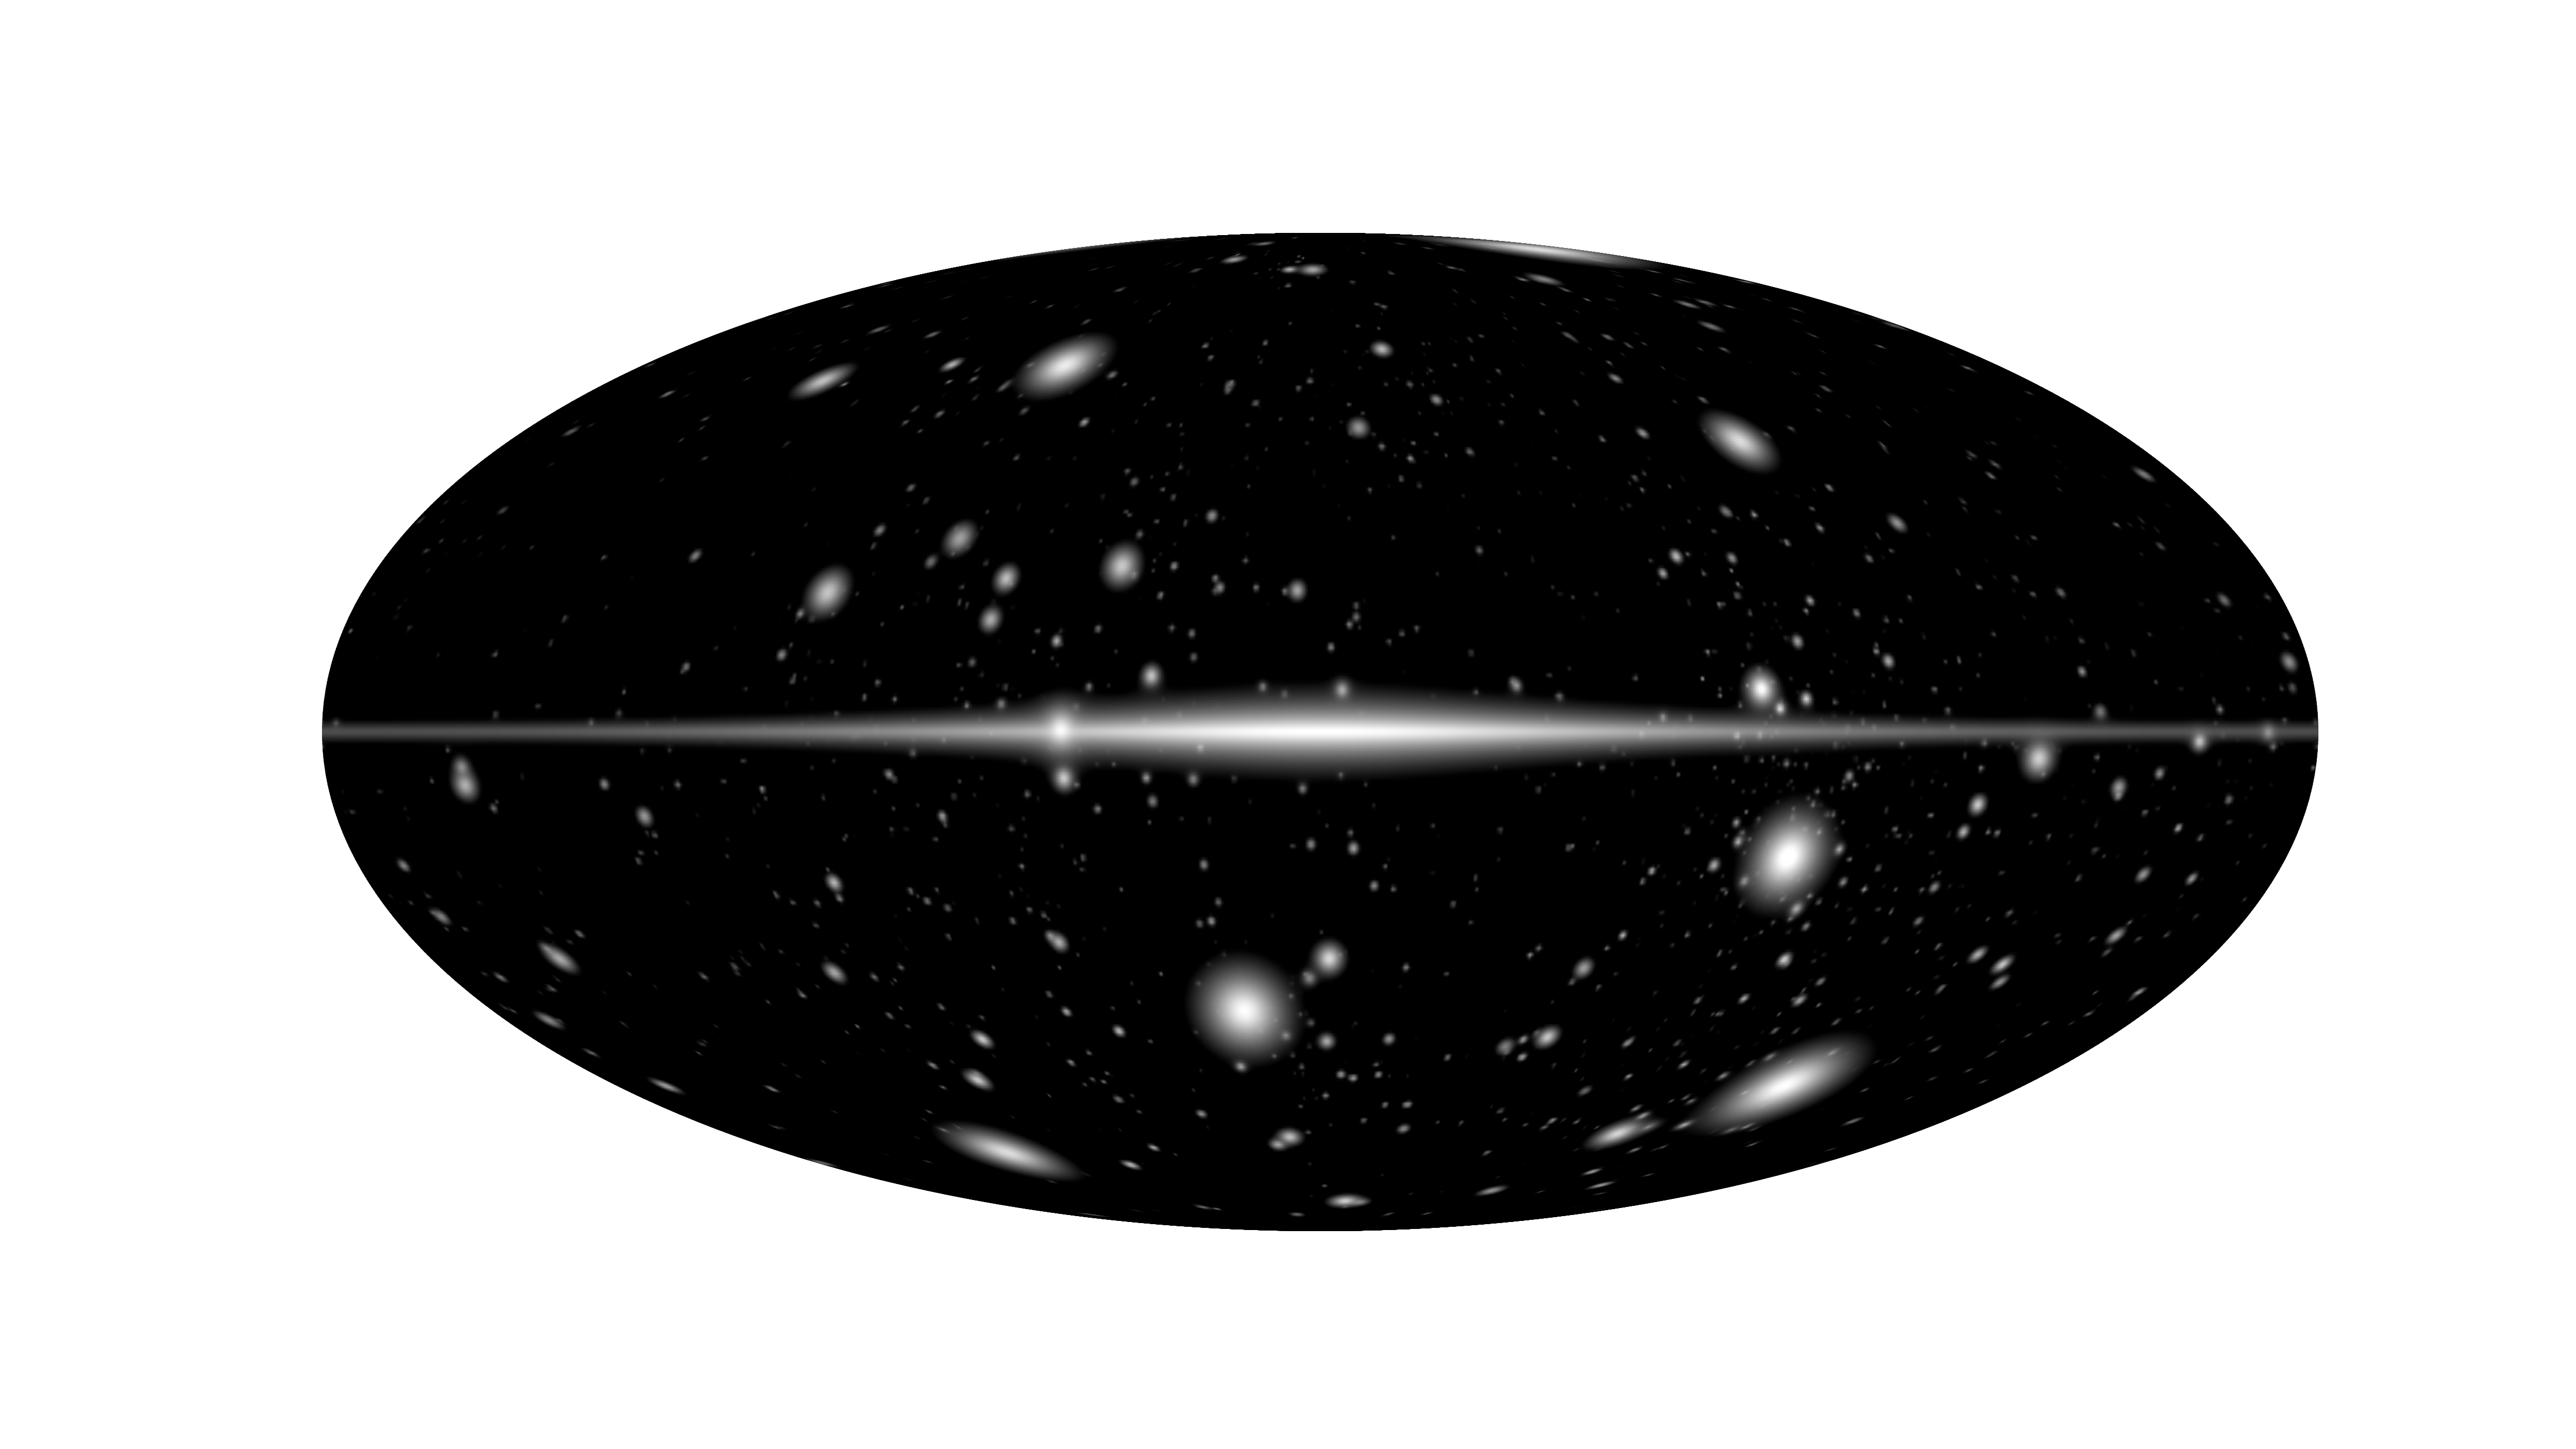
\includegraphics[width=\linewidth]{images/mollweide-density-with-haloes.png}
            \caption[Plausible $\Lambda$CDM dark matter subhalo population as ``seen'' from the Sun]{Plausible $\Lambda$CDM dark matter subhalo population as ``seen'' from the Sun. The subhalos are modeled as Plummer spheres, with their light integrated along the line of sight from the Sun and scaled according to the total halo mass. Overlaid is the integrated surface light density profile of the Milky Way's stellar disk, modeled with a Miyamoto-Nagai potential. DM simulation from Boldrini et al. (in prep). }
            \label{fig:mollweide-density-with-haloes.png}
        \end{figure}

        There is considerable modeling work on gap formation in stellar streams. While we aim to make theoretical predictions for the expected number of gaps, these must be set in the context of a realistic Milky Way potential that includes known time-dependent and non-axisymmetric features. To date, most studies have examined either subhalo encounters in isolation \citep{2013ApJ...775...90C,2015MNRAS.450.1136E,2016MNRAS.463..102E,2016MNRAS.457.3817S,2024arXiv241213144A,2025arXiv250207781L} or the effect of the Galactic bar alone \citep{2016MNRAS.460..497H,2016ApJ...824..104P,2017NatAs...1..633P,2023A&A...678A.180T}. However, it is known that perturbations from baryonic structures can also generate gap-like signals, potentially mimicking the effects of DM subhalos \citep{2020ApJ...891..161I}. To correctly frame the inference problem, the false positive rate must therefore be quantified and calibrated.

        Ultimately, the inversion of this problem is a case study in Bayesian hierarchical modeling \citep{2020sdmm.book.....I}. Each gap detection is under-determined \citep{2015MNRAS.450.1136E}: even in the absence of measurement uncertainties, a single gap cannot uniquely constrain the perturber's mass, size, time of impact, and relative velocity simultaneously. Nevertheless, with a sufficiently large sample of gaps and posterior distributions for each encounter, we can begin to infer statistical properties of the DM subhalo population.

        This is a challenging problem. We must account for other astrophysical processes that can erase gap signatures or create false positives, quantify their rates, and embed them in a hierarchical inference framework. The application of such an analysis to the Milky Way will require extremely high-quality data, which may be achievable with future LSST observations and the final Gaia data releases.

        As highlighted in Chapter~5, the coherence of a stream is crucial for gap survival, and this must be modeled accurately to avoid overestimating gap counts. In order to obtain proper predictions, we must accurate model stream generation. While full $N$-body simulations would be the most physically accurate way to model internal cluster dynamics and their mapping into streams, they are computationally prohibitive for the parameter space we must explore. Capturing variations in the Galaxy's potential, cluster internal dynamics, orbital initial conditions, DM subhalo populations, and the properties of multiple streams could require computing tens of thousands of stream realizations. $N$-body simulations have long been at the avant-garde of computational astrophysics, often driving innovations in both hardware and software. A notable example is the GRAPE (GRAvity PipE) series of special-purpose computers developed for gravitational $N$-body problems \citep{1991PASJ...43..841F,1997ApJ...480..432M}. For over a decade, GRAPE systems enabled simulations that would have been prohibitively slow on general-purpose hardware, pushing the limits of the field. Eventually, advances in general-purpose graphics processing units (GPUs) offered comparable performance with greater flexibility, leading to the widespread adoption of GPU-accelerated $N$-body codes \citep{2012MNRAS.424..545N,2015MNRAS.450.4070W}. Despite these hardware revolutions, the computational cost of the large ensembles of simulations required for our purposes remains high.

        Several methods have been developed to avoid the need for full $N$-body modeling. The ``streak-line'' method \citep{2012MNRAS.420.2700K} approximates streams as having the same orbital parameters as their progenitor. The action-angle formalism of \citet{2011MNRAS.413.1852E} describes each stream star as having a small offset from the progenitor's Hamiltonian, expressible via a second-order Taylor expansion. \citet{2014ApJ...795...95B} used this to develop the ``particle-spray'' method, which improves upon the streak-line model by introducing velocity dispersion into the streams. As noted by \citet{2015MNRAS.452..301F}, this is one of the most elegant stream modeling approaches to date.

        \citet{2015MNRAS.452..301F} also developed a prescriptive stream-generative model, fitting analytic functions to escape rates measured from $N$-body simulations. This method operates on the dynamical timescale of the Galaxy rather than the cluster's internal timescale, greatly speeding up computations.  

        The internal dynamics of globular clusters involve a rich range of processes \citep{1997A&ARv...8....1M}. While particle-spray and semi-analytic methods can be extremely efficient, extrapolating beyond the regime covered by their $N$-body calibrations can be risky. However, machine learning techniques \citep{2023ApJ...959...99T} offer a promising way to emulate $N$-body simulations without assuming a specific parametric form, providing both flexibility and speed.

        In summary, with upcoming improvements in both data quality and modeling techniques, there is strong potential to make significant progress in this field. %Depending on computational constraints, I may either adopt an existing stream simulation method in place of \texttt{tstrippy} or implement a particle-spray approach within it.

    \subsection{The bulk gravitational field of the MW}
        At the onset of this thesis, our aim was to investigate large-scale features of the Milky Way such as spiral arms, the Galactic bar, giant molecular clouds, and satellite galaxies and their effect of globular cluster streams. Each of these components represents a potential avenue for further study.  

        In particular, we are interested in the role of the Galactic bar. Previous works have shown that the bar can induce chaotic orbits, causing stellar streams to ``fan out'' more than they otherwise would \citep{2016ApJ...824..104P,2020ApJ...889...70B}. Our preliminary investigation, based on the simulations of \citet{2023A&A...673A..44F}, revealed several intriguing effects. As noted by other authors \citep[see Fig.~9 of][]{2025NewAR.10001713B}, the bar can generate large underdensities along streams. Our own simulations suggest additional signatures beyond this.  

        The total mass, orientation, and length of the bar have been constrained in previous studies, though significant uncertainties remain. Most notably, the bar pattern speed (its angular velocity) still has two plausible regimes: slow or fast rotation \citep{2015MNRAS.450.4050W,2016ARA&A..54..529B,2023MNRAS.520.4779L,2024MNRAS.528.3576V}, not to mention the effect of the the bar deceleration \citep{2024A&A...690A.147H} on the streams. 

        We are conducting new experiments to explore whether stellar streams can help break some of these degeneracies. As an example, Fig.~\ref{fig:pal5_with_bar} shows simulations of the Palomar~5 stream for a range of bar pattern speeds. In some cases, the bar splits the stream and creates prominent gaps; in others, it shifts part of the stream off its typical track; in yet others, it suppresses the stream's growth entirely, keeping debris bound near the progenitor cluster.  

        \begin{verbatim}
            VIDEO: Pal5_longmurali_5000_monte_carlo_002_white_bg.mp4
        \end{verbatim}

        \begin{figure}
            \centering
            \begin{tabular}{ccc}
                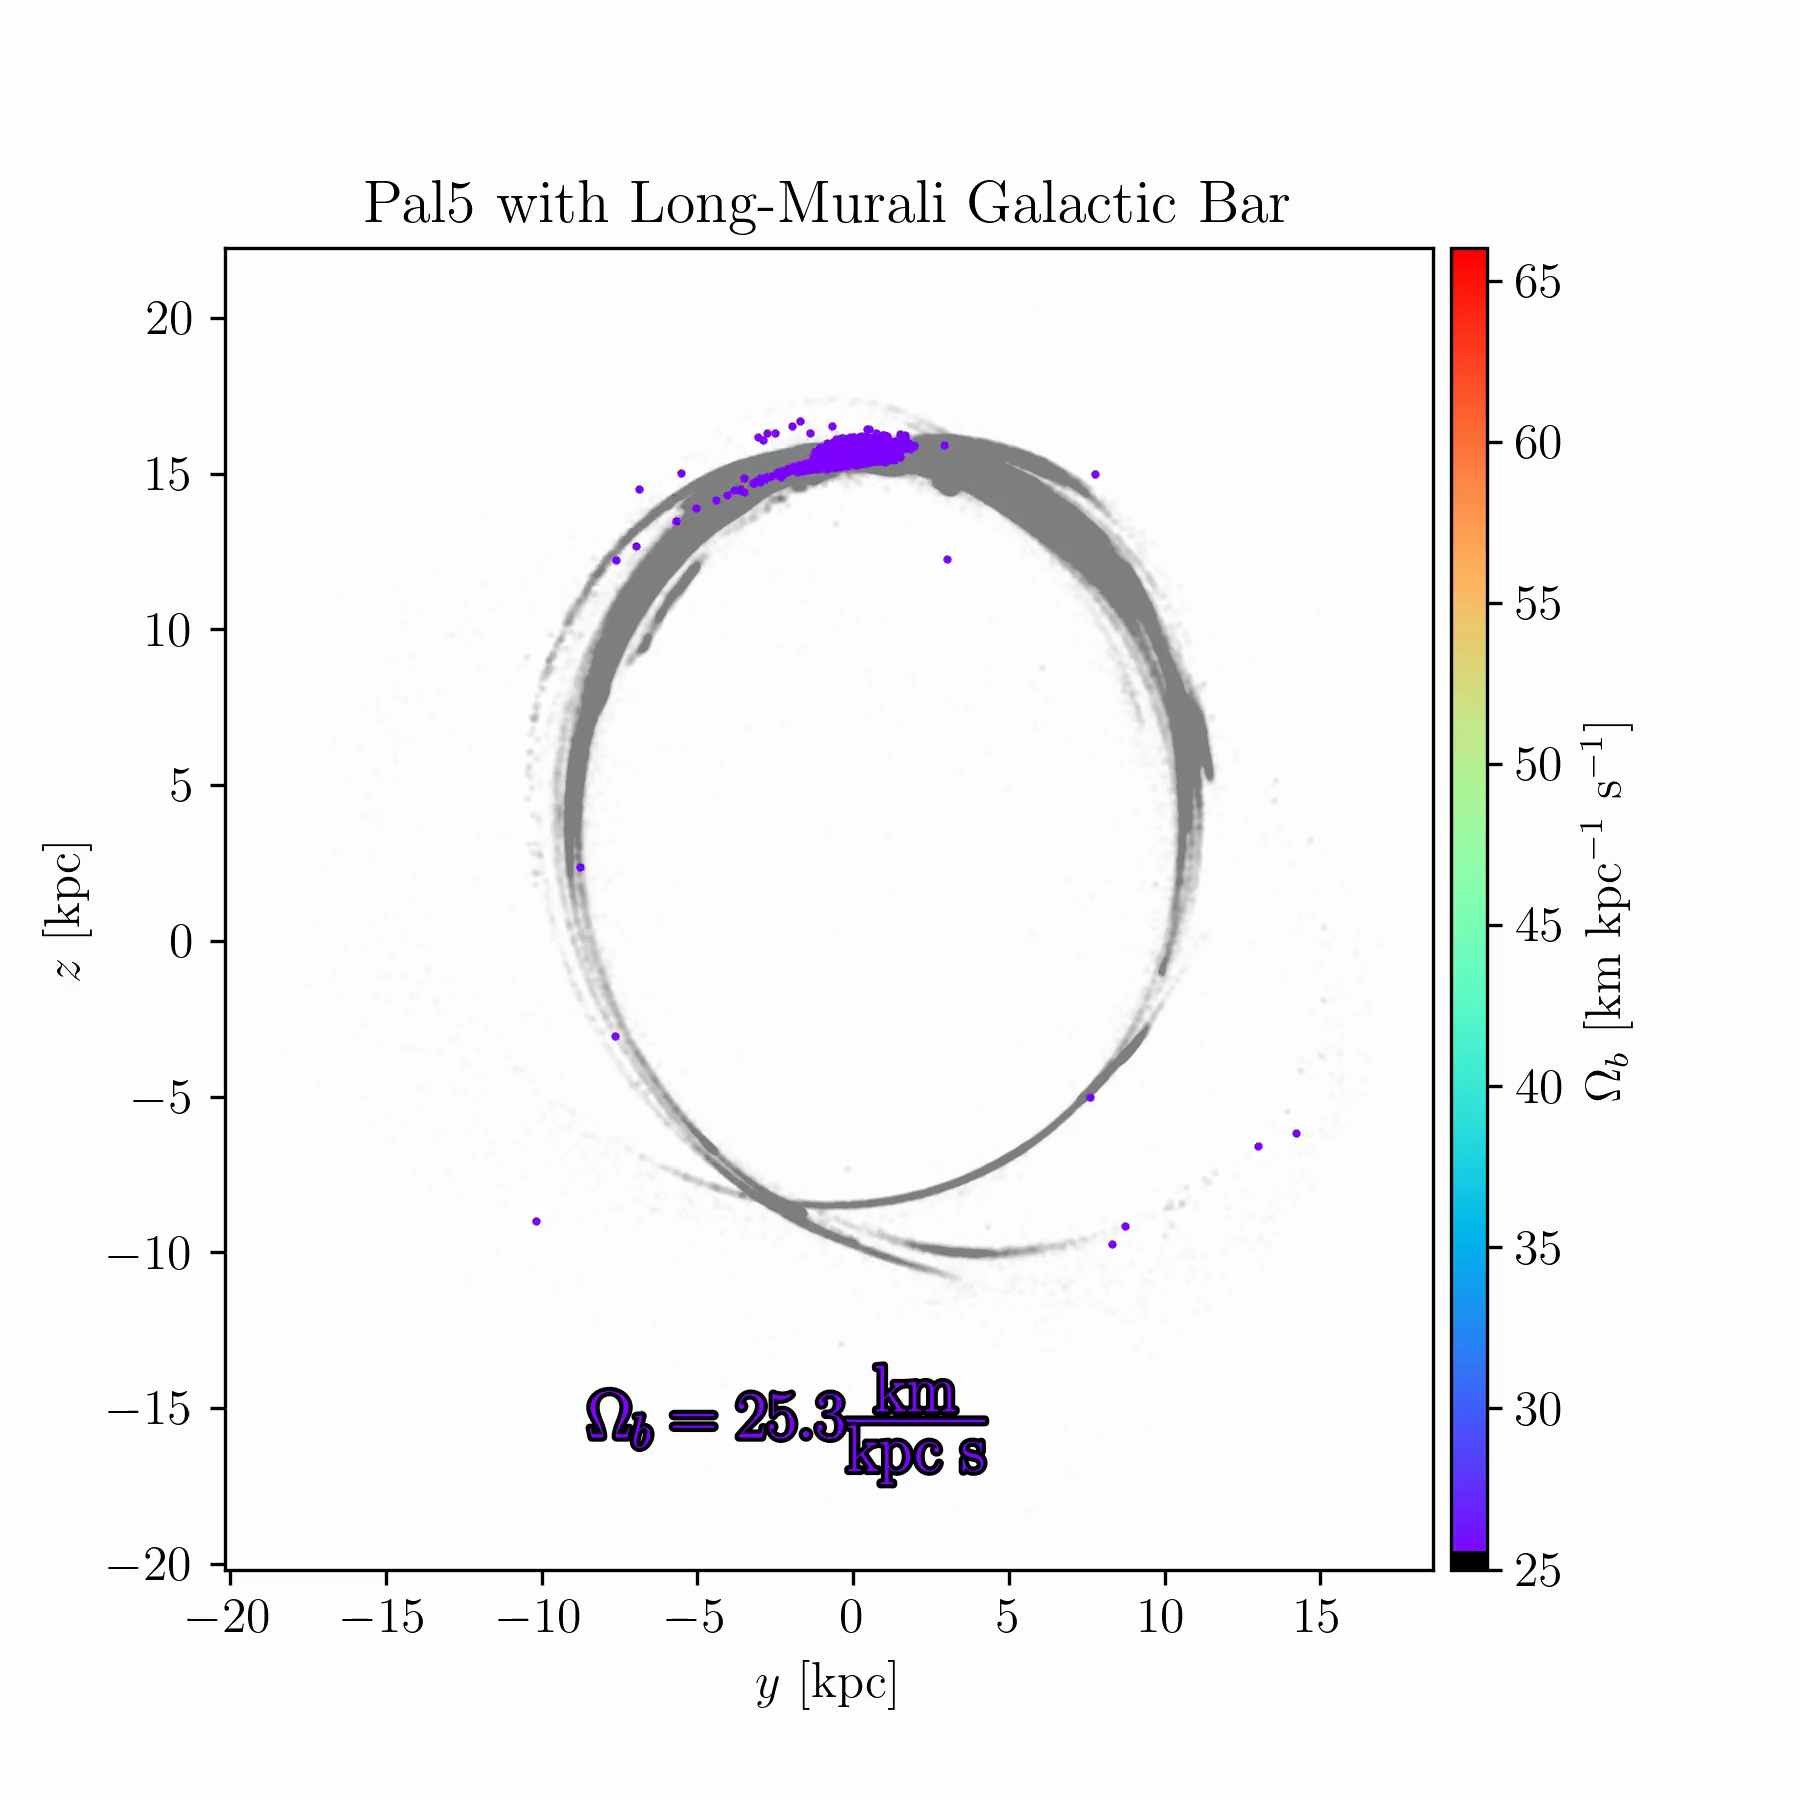
\includegraphics[width=.32\linewidth]{images/frame_0002.png}&
                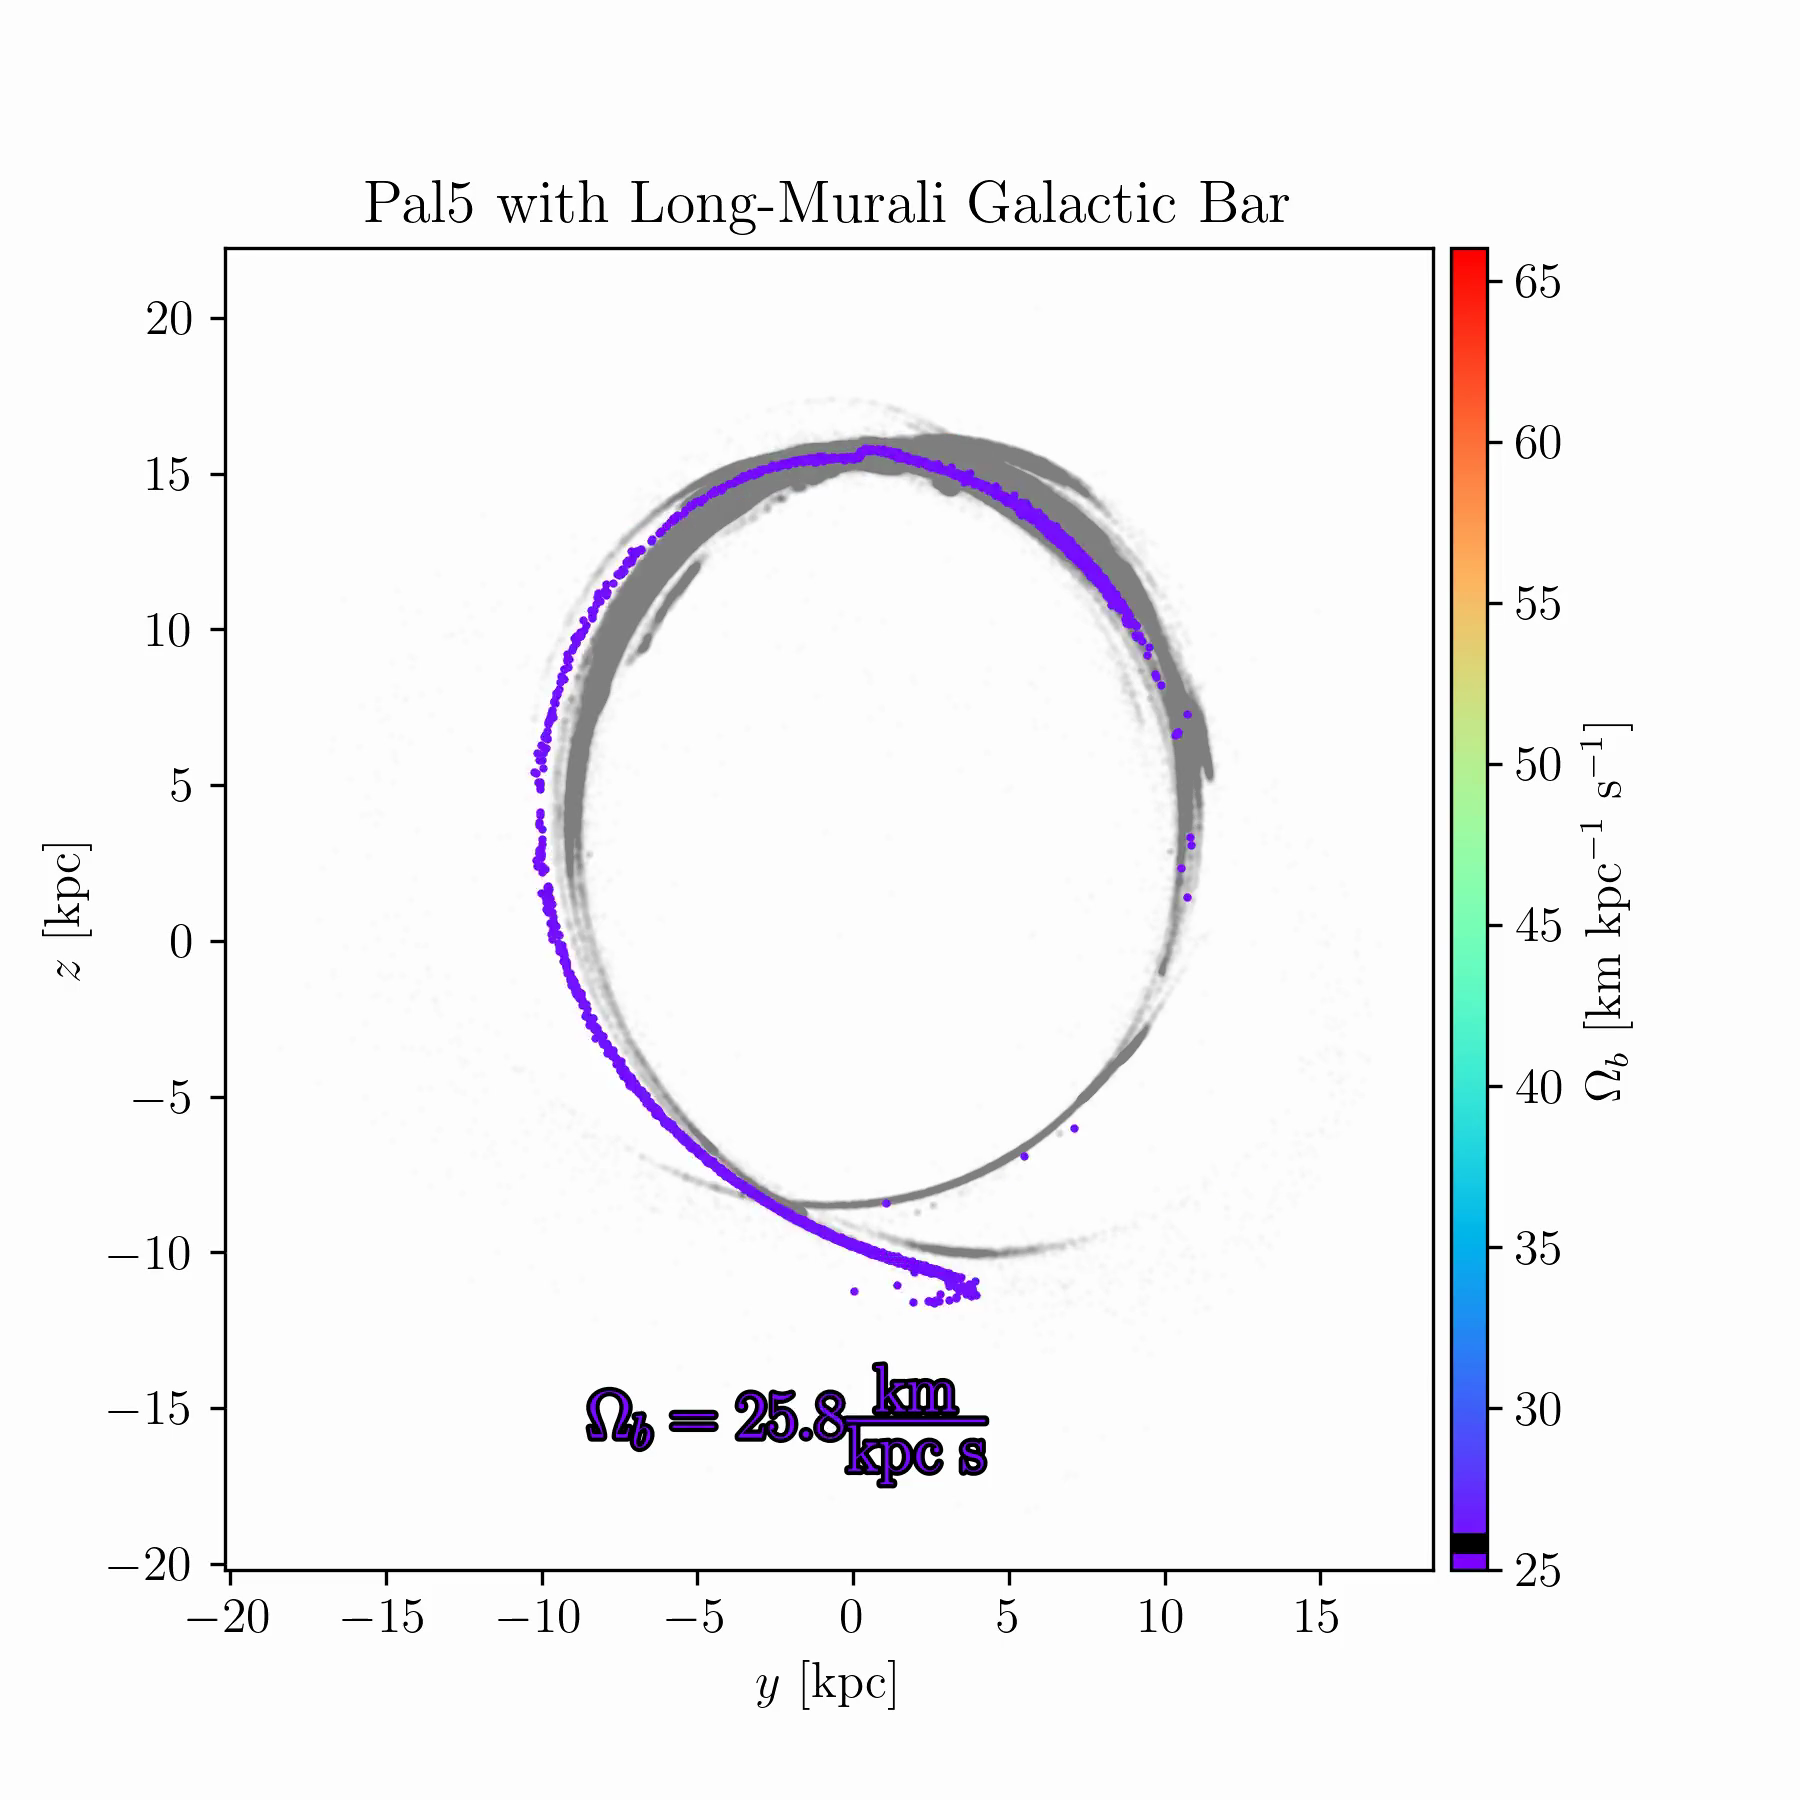
\includegraphics[width=.32\linewidth]{images/frame_0004.png}&
                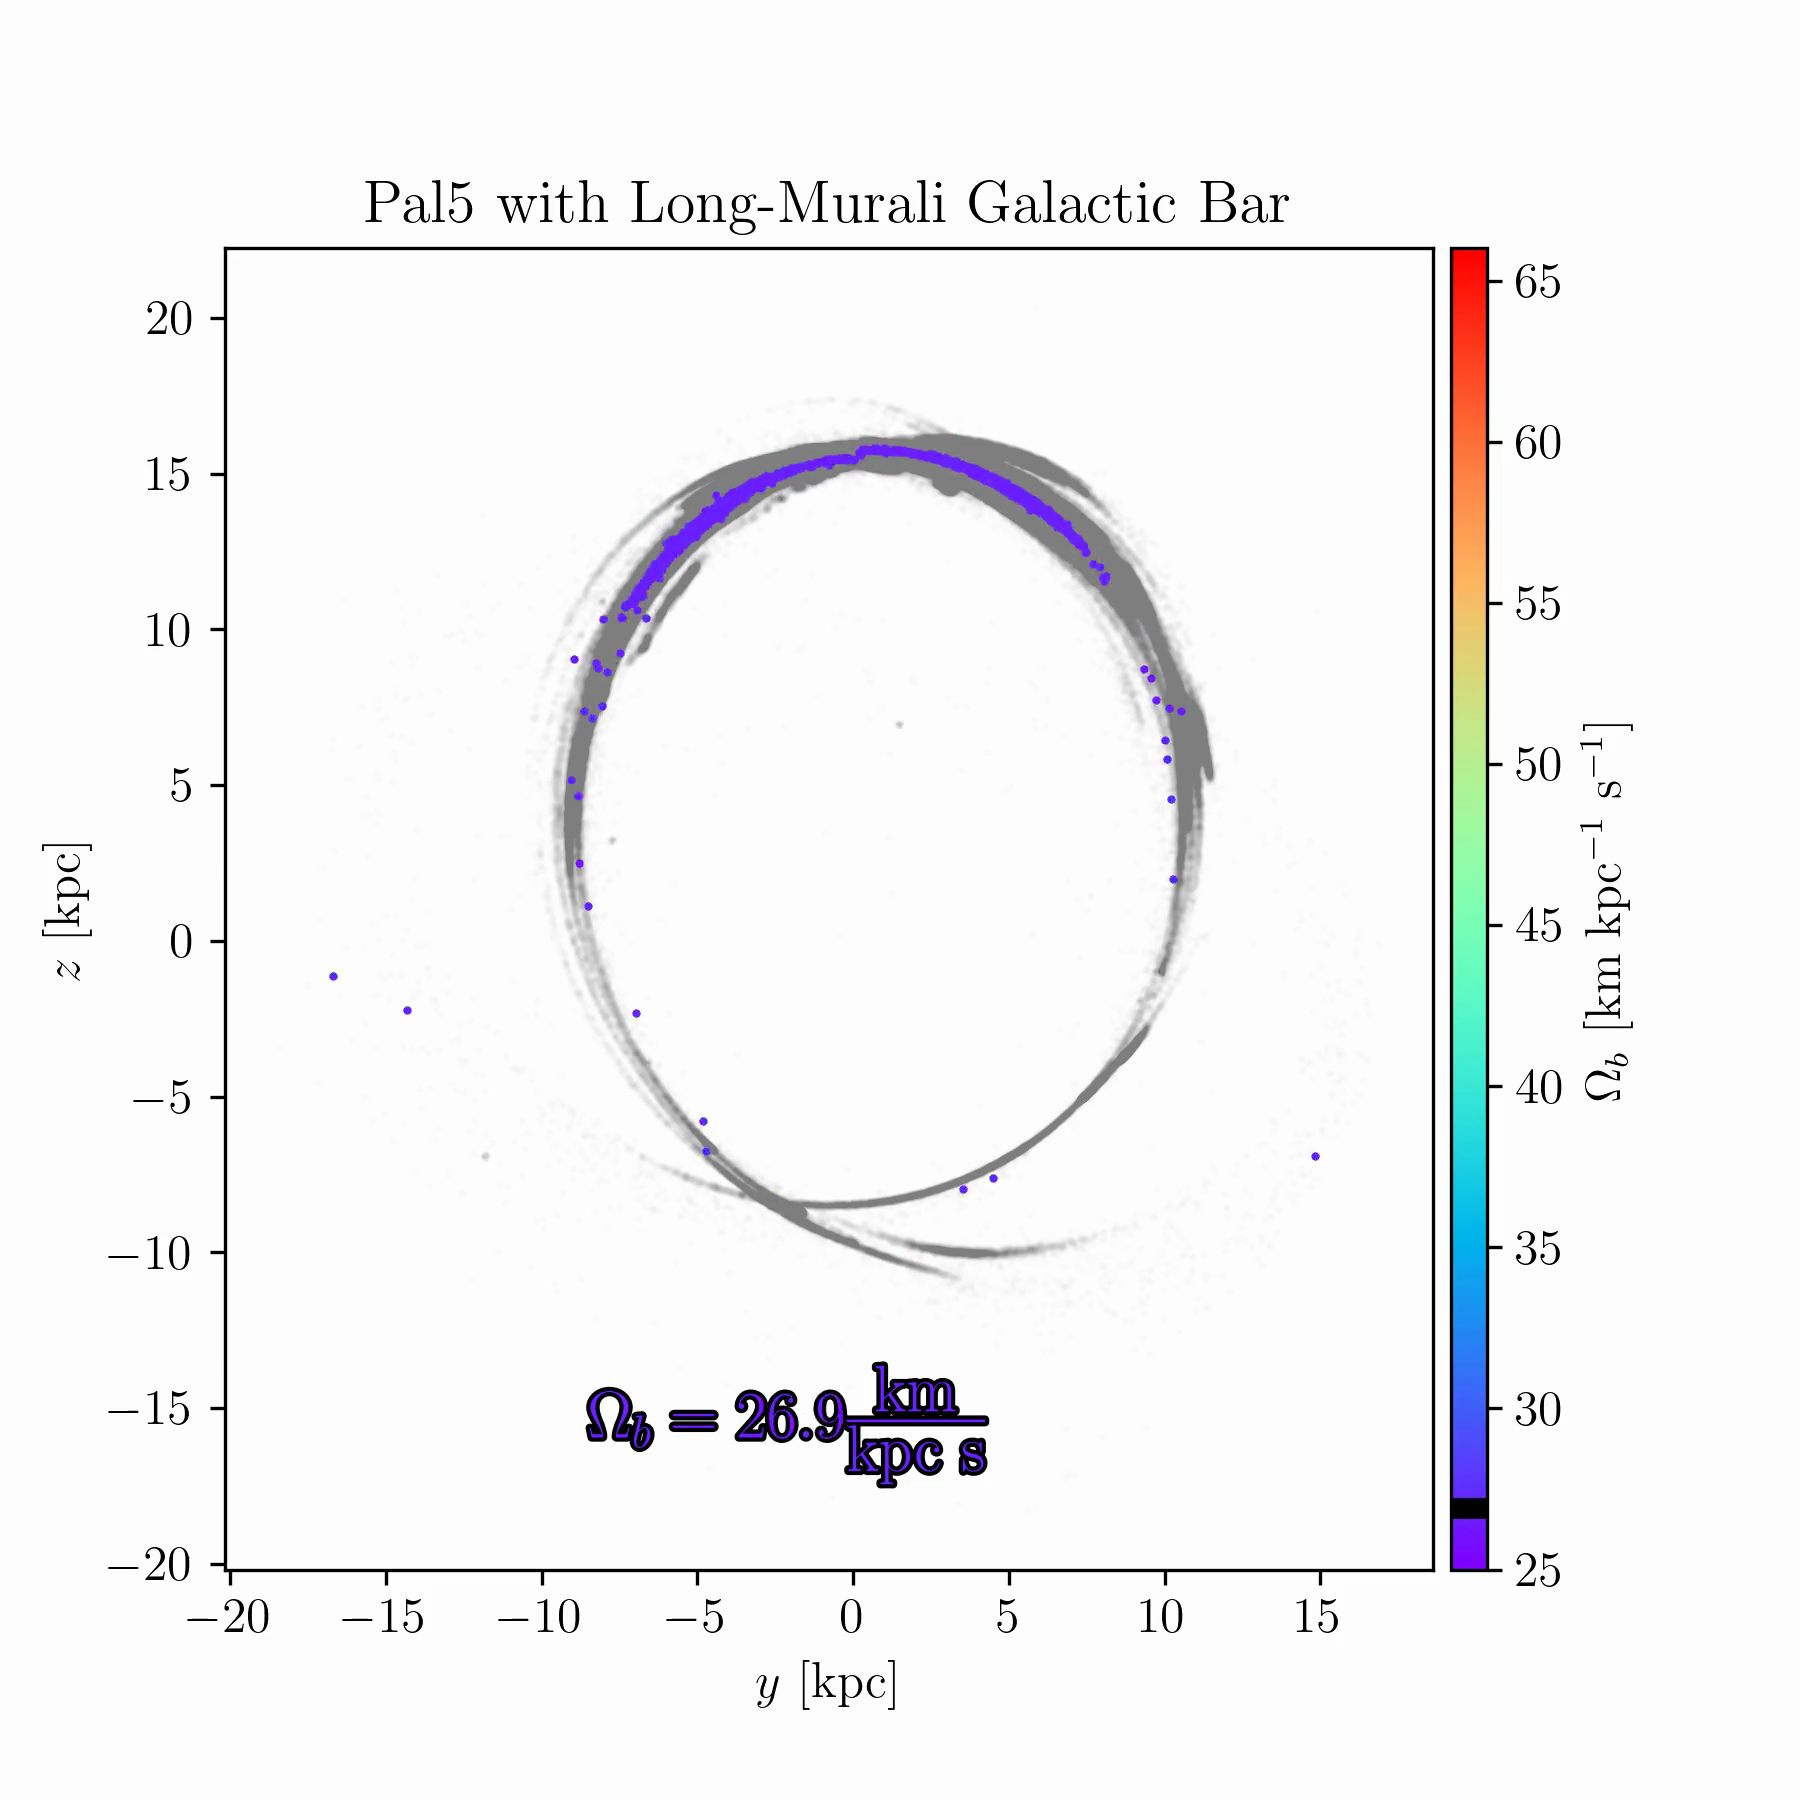
\includegraphics[width=.32\linewidth]{images/frame_0008.png}\\
                
                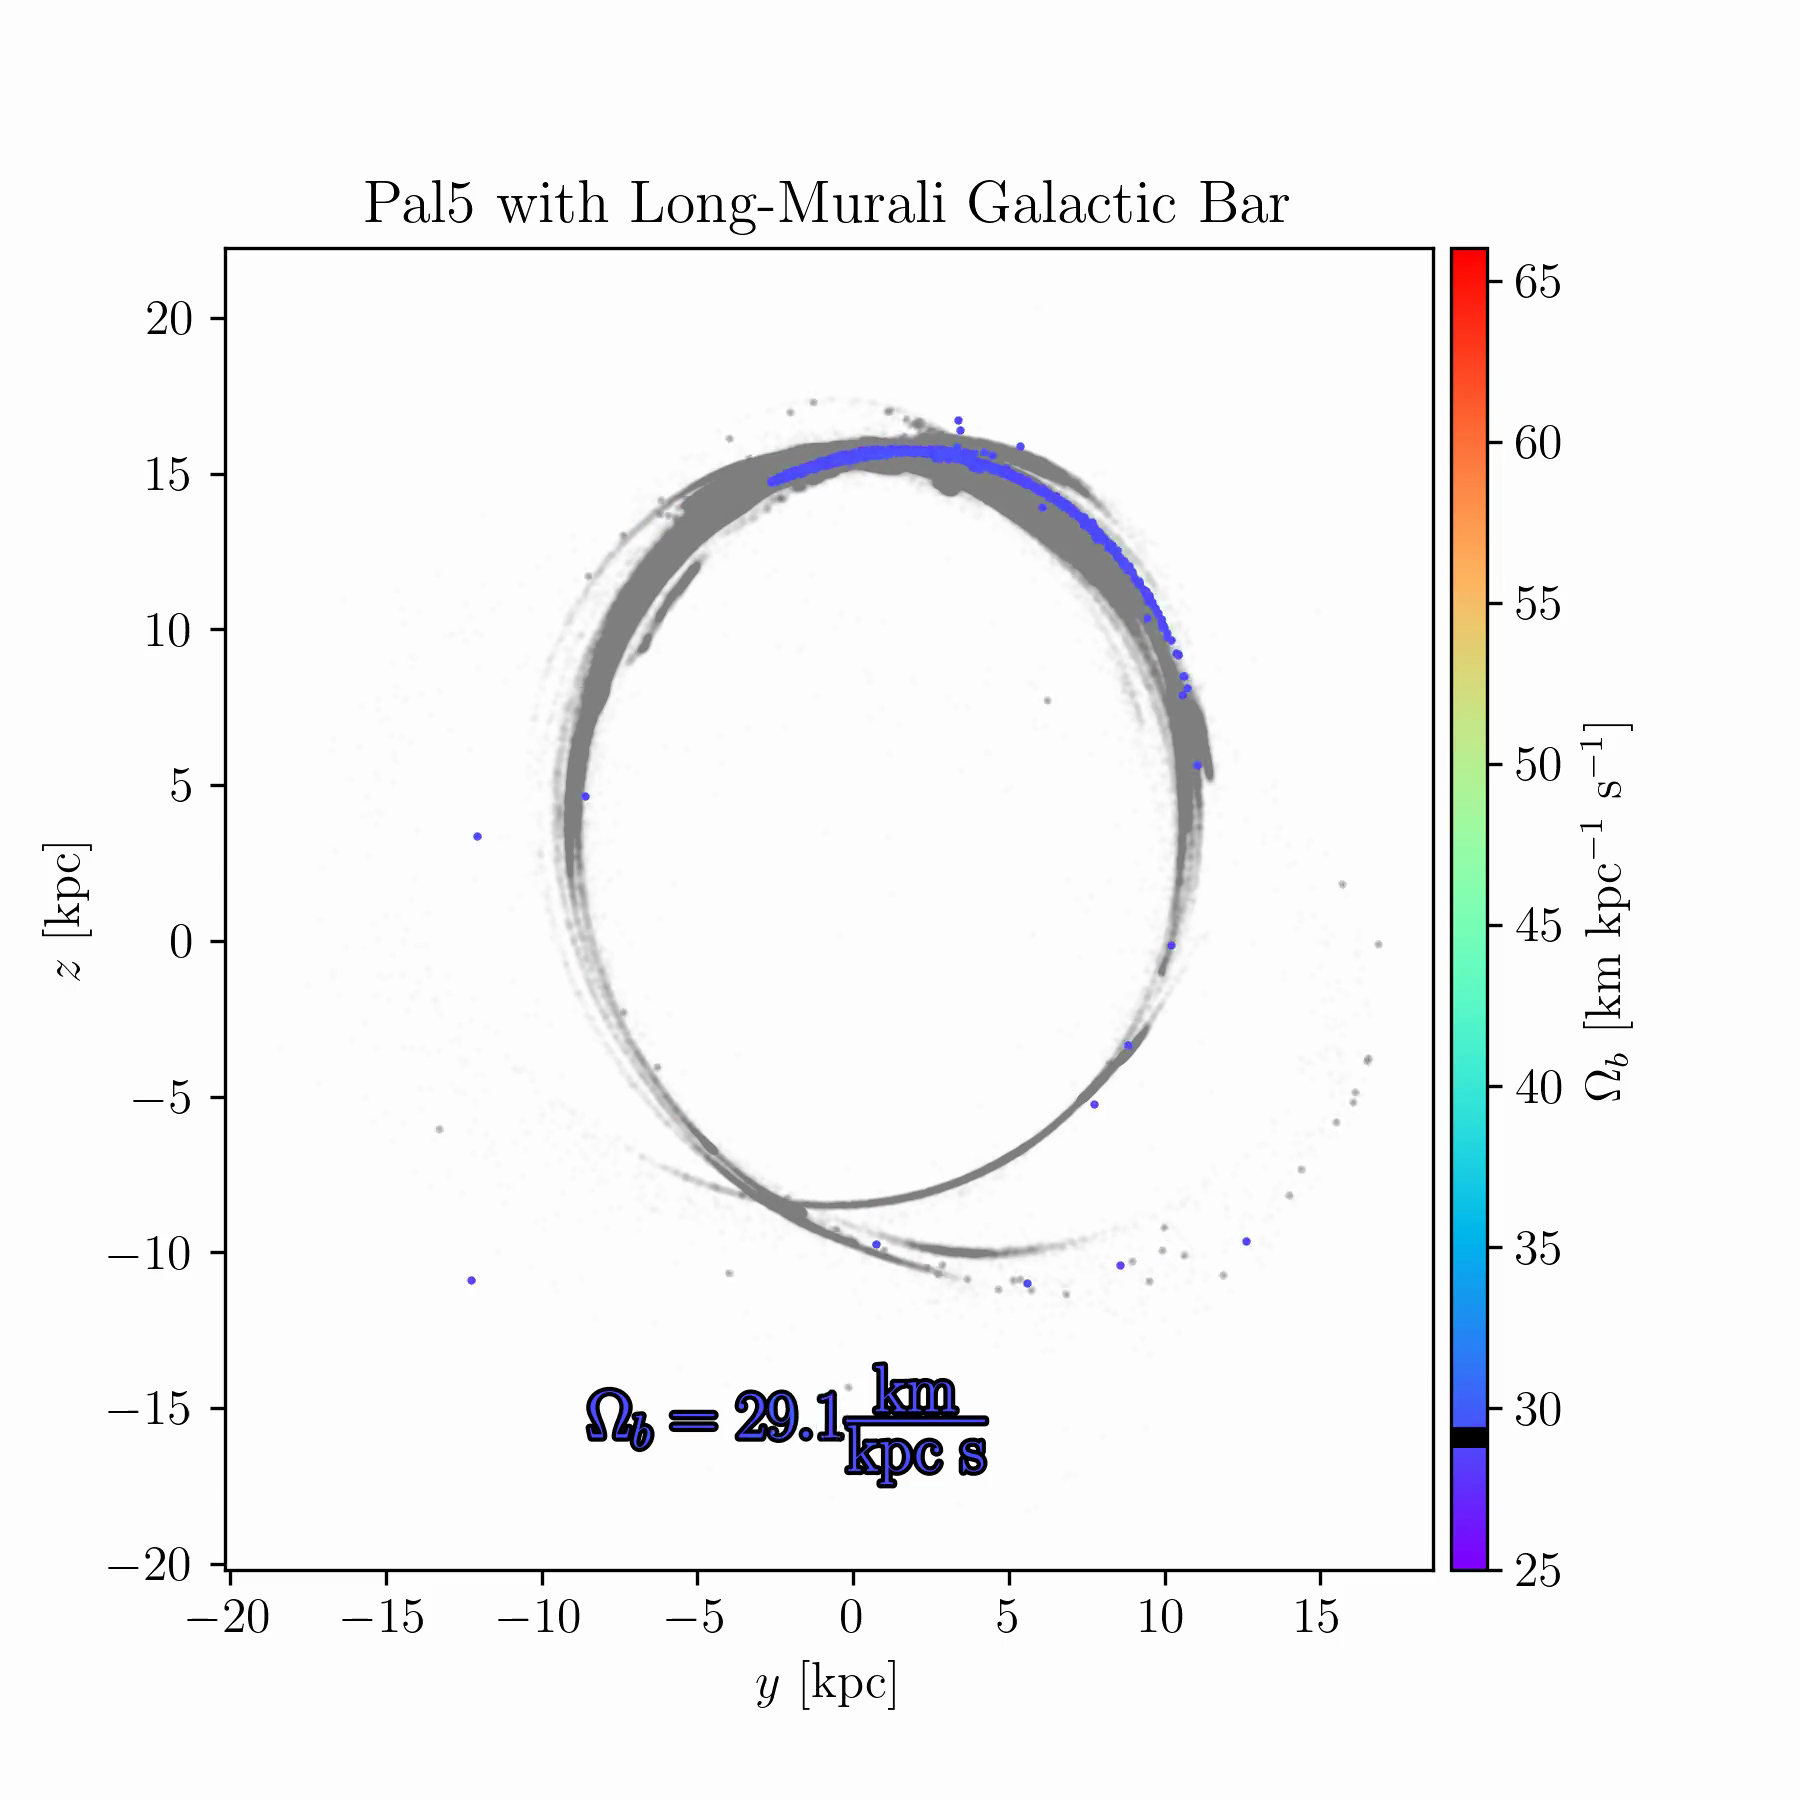
\includegraphics[width=.32\linewidth]{images/frame_0016.png}&
                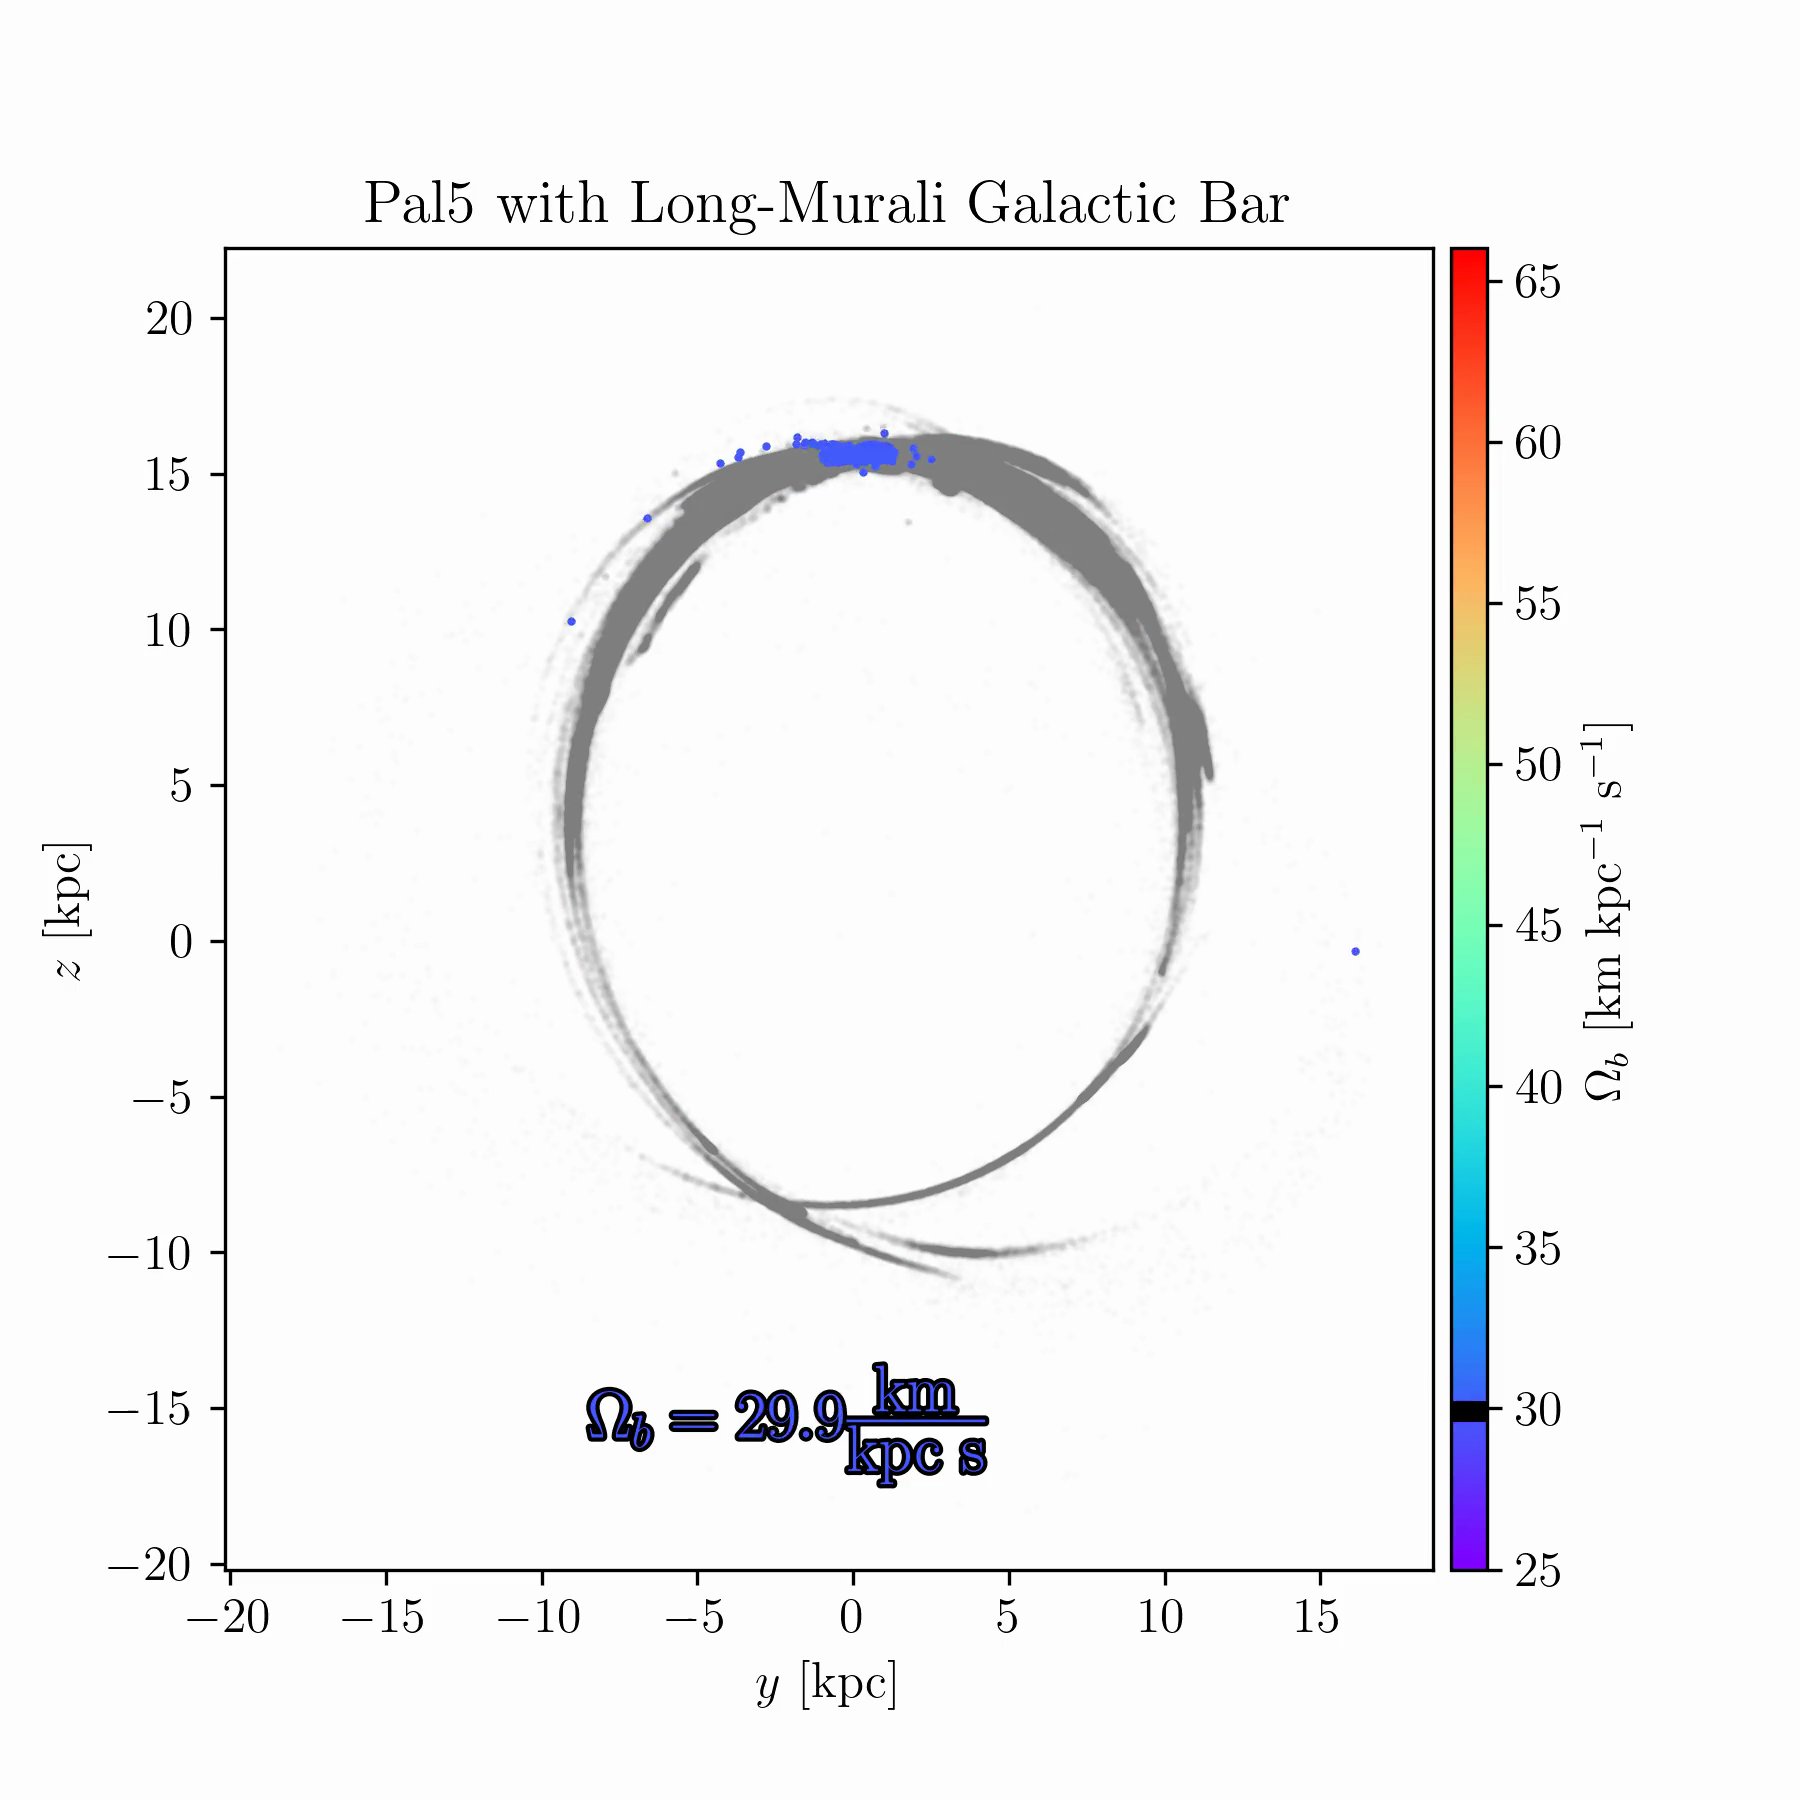
\includegraphics[width=.32\linewidth]{images/frame_0019.png}&
                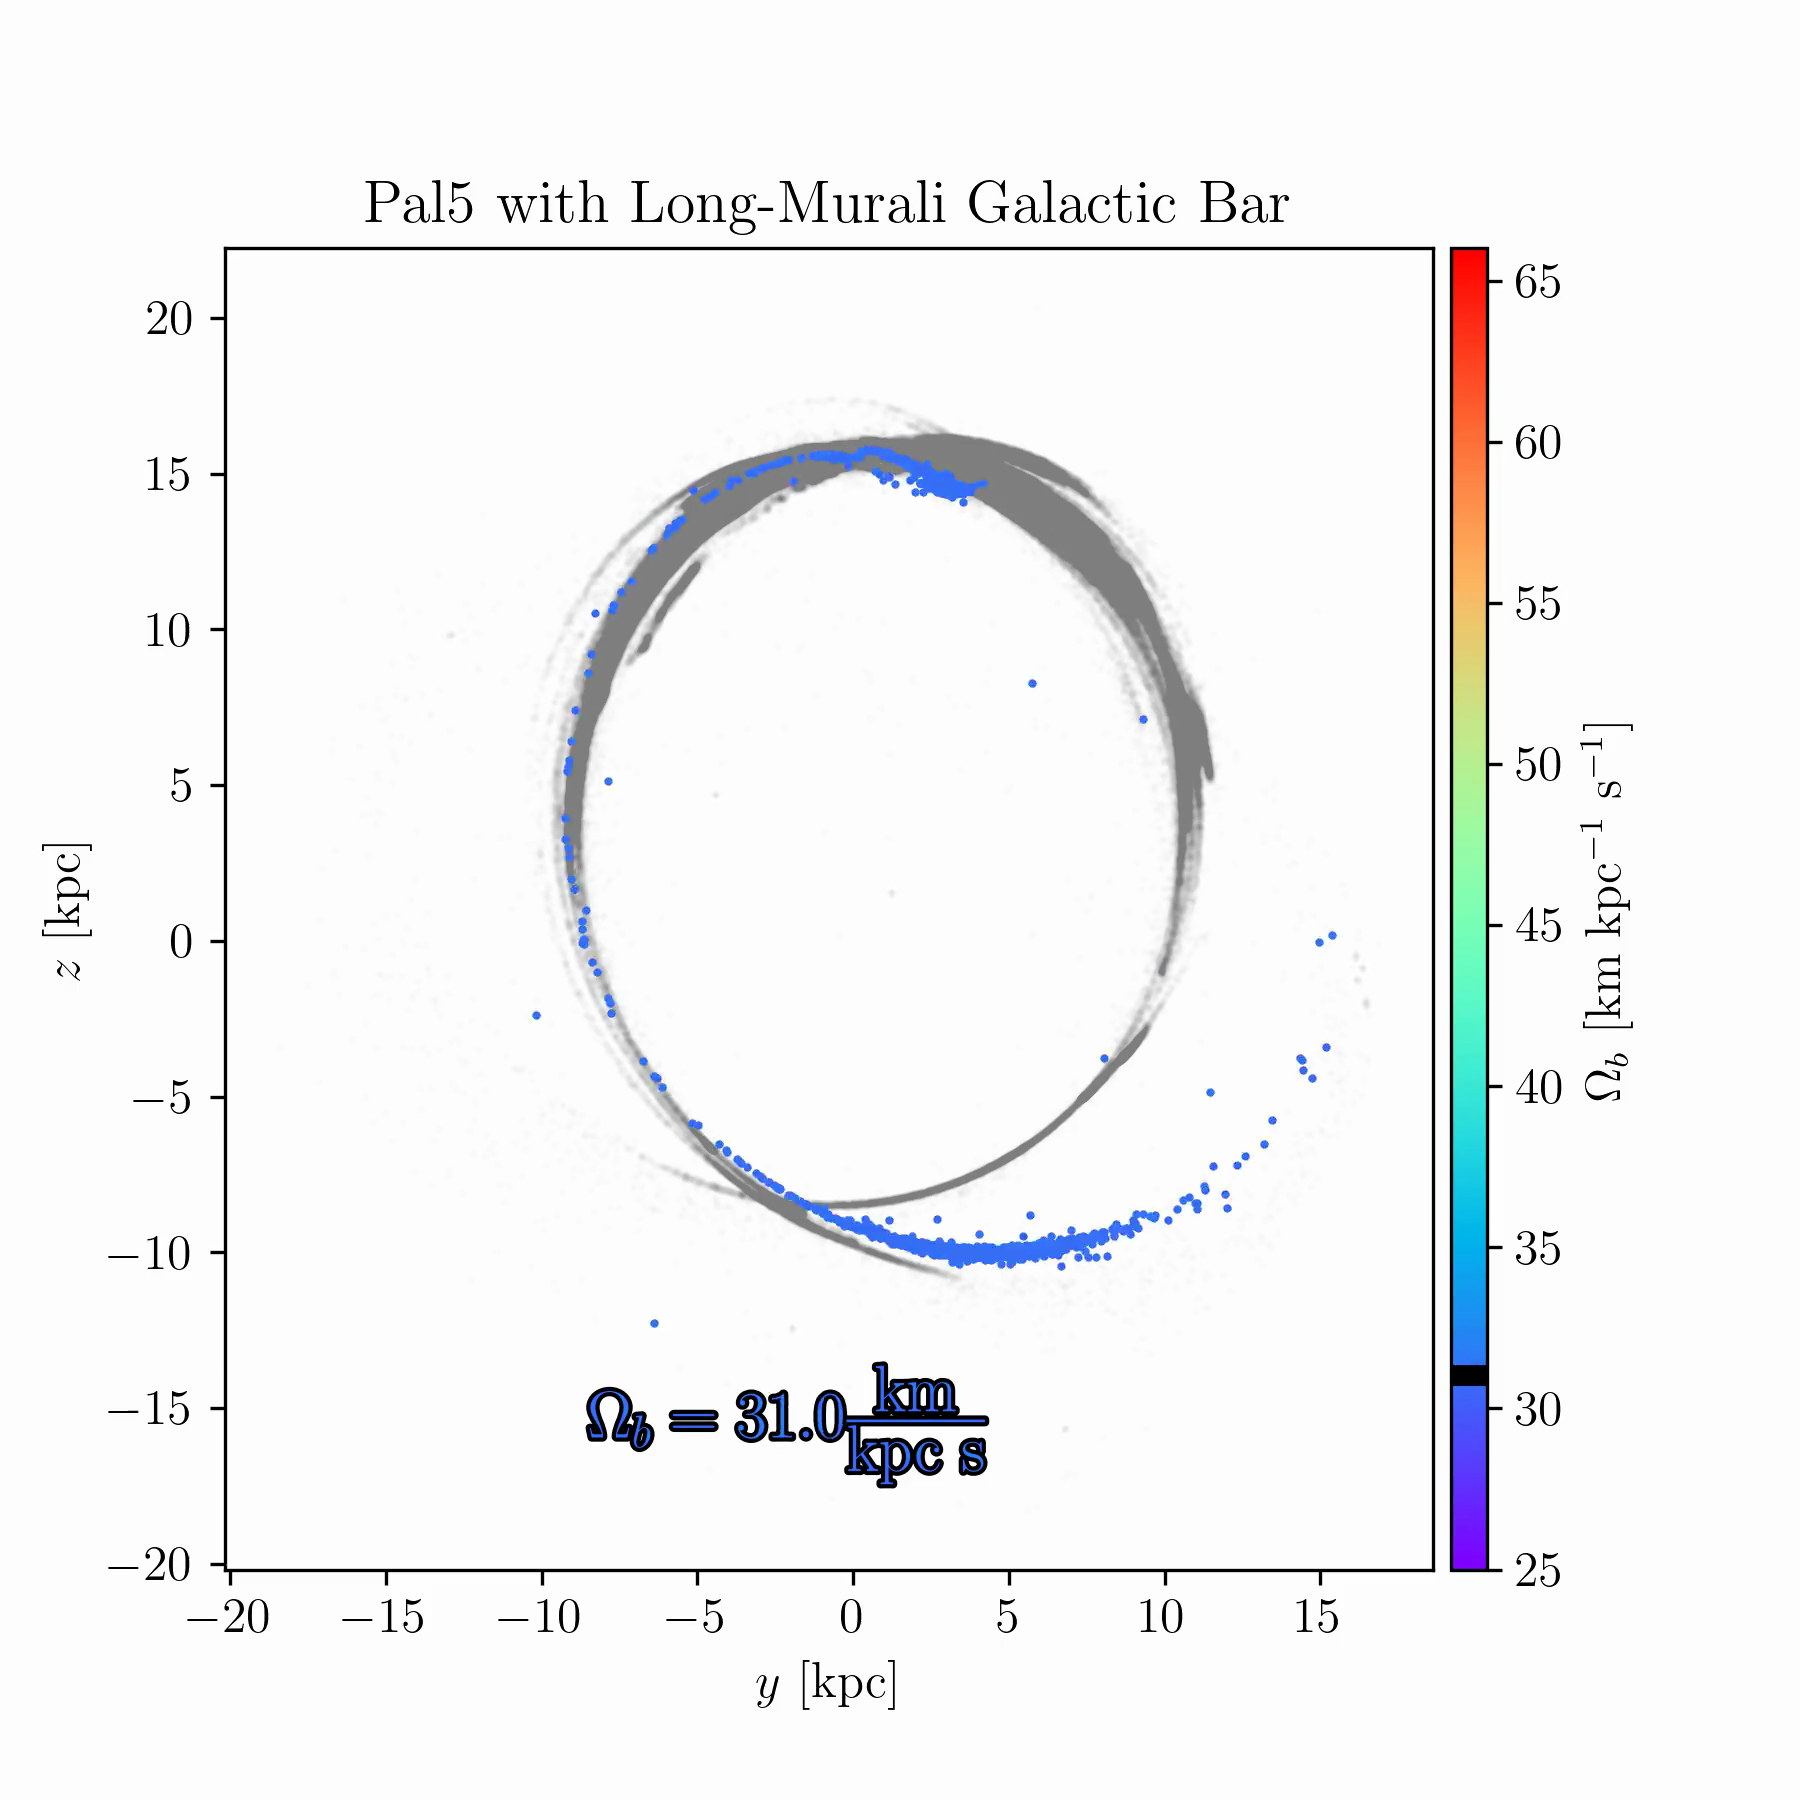
\includegraphics[width=.32\linewidth]{images/frame_0023.png}\\
                
                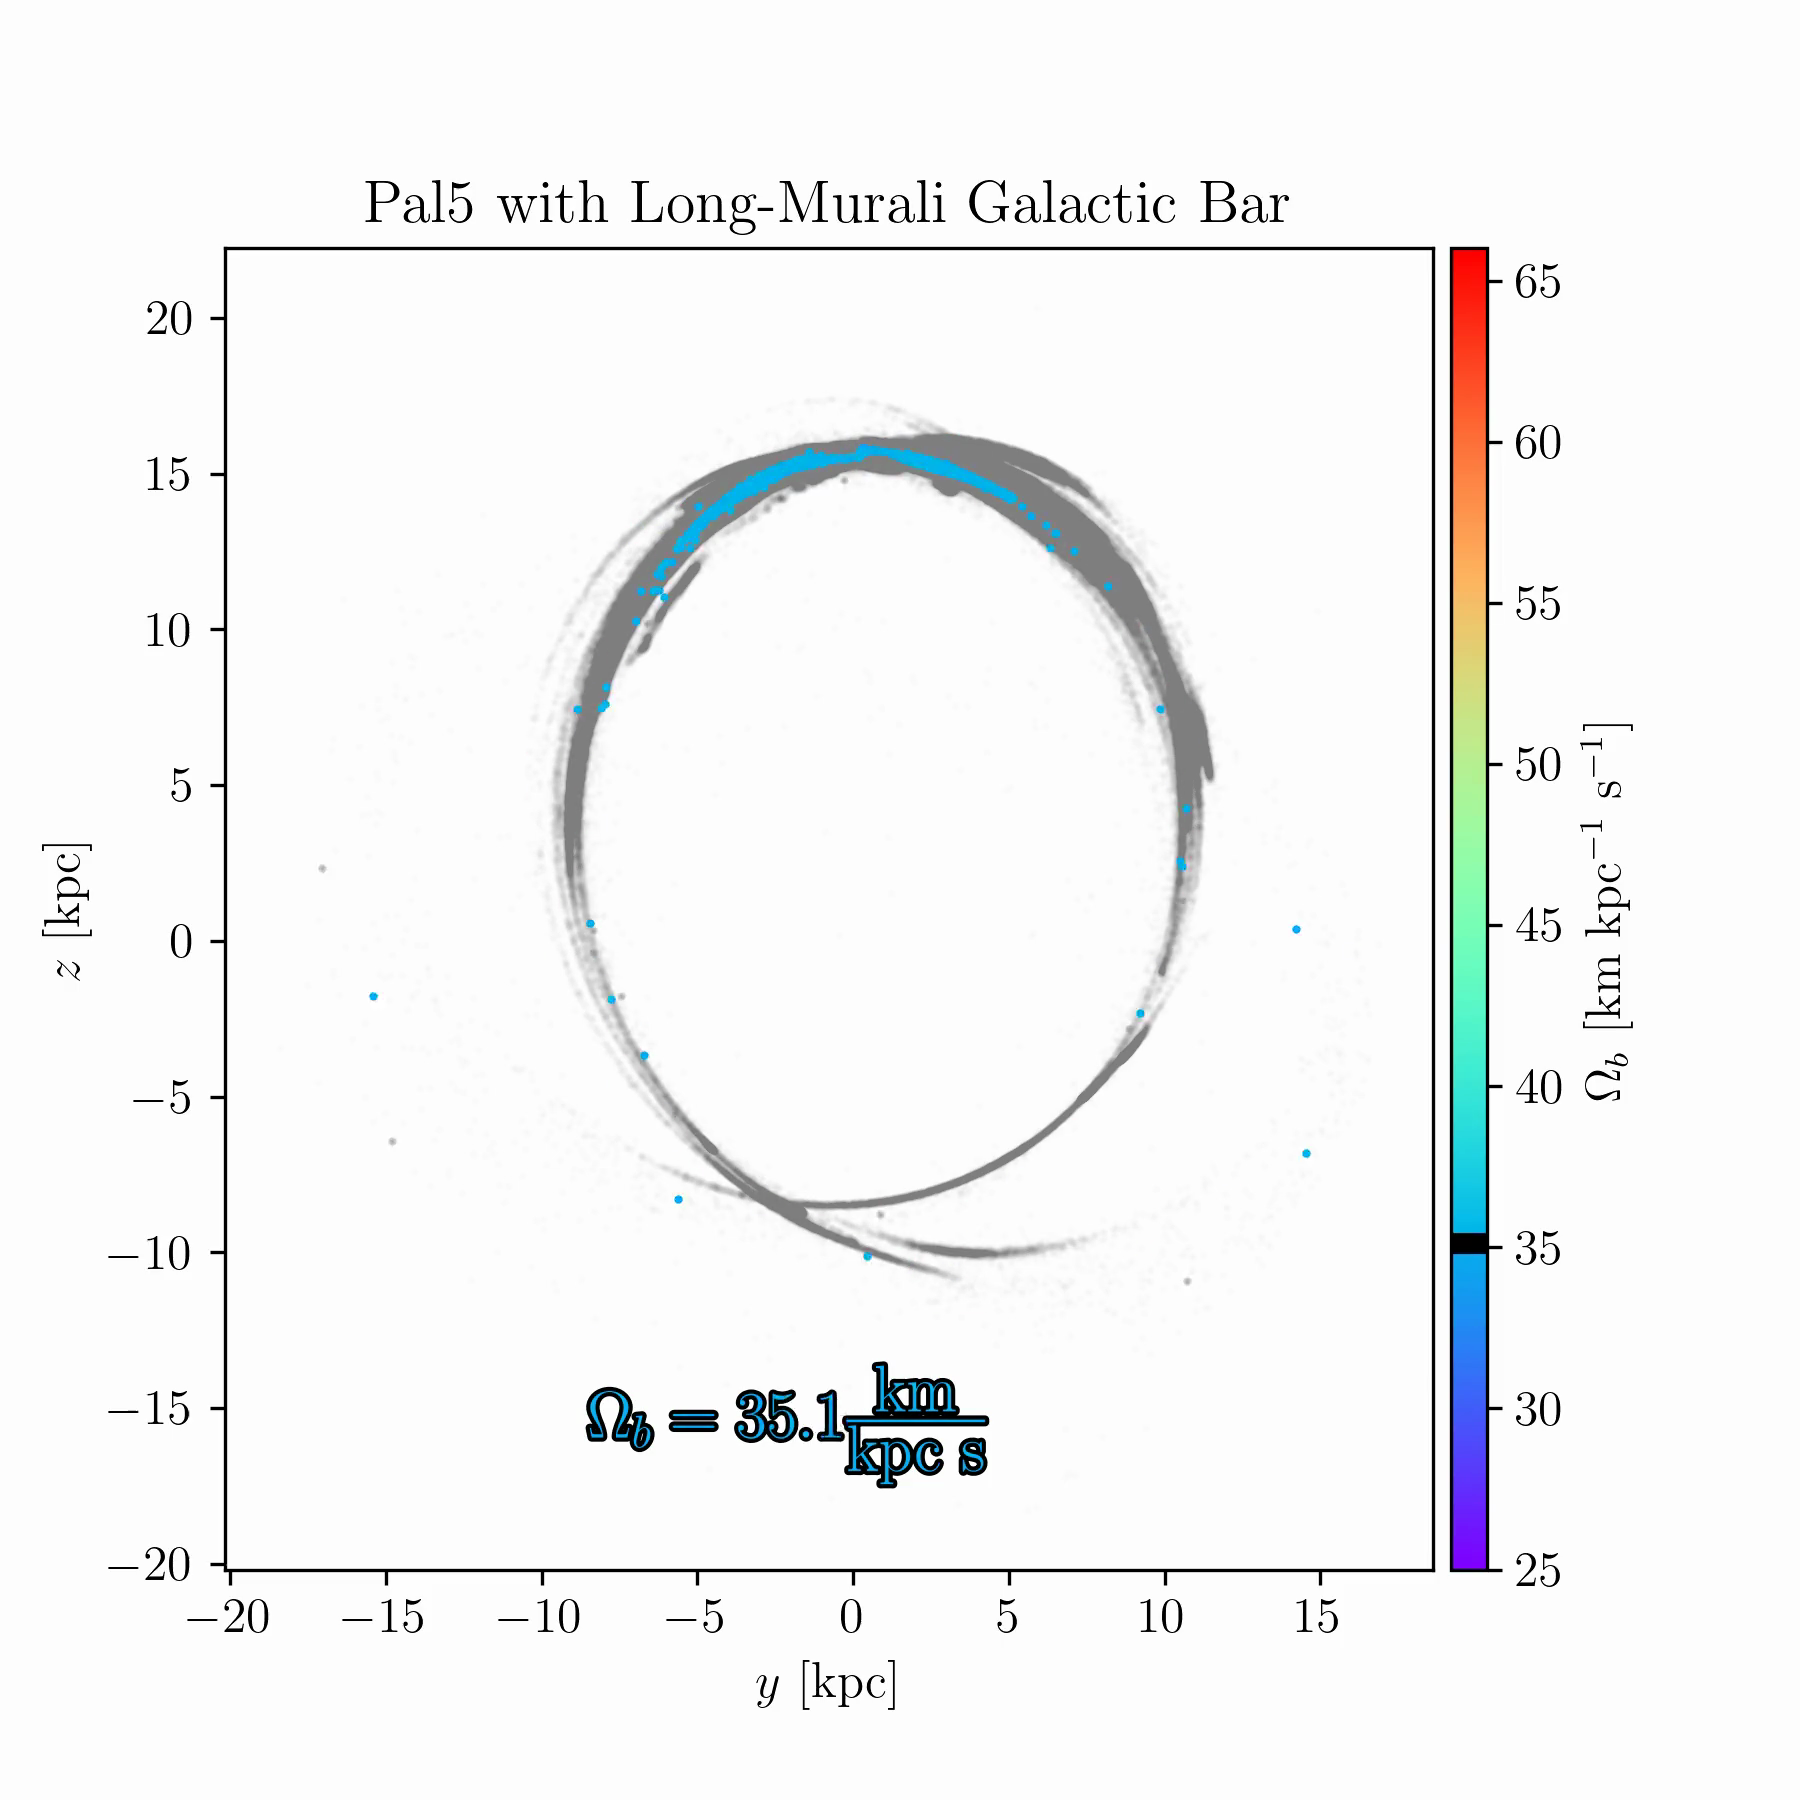
\includegraphics[width=.32\linewidth]{images/frame_0038.png}&
                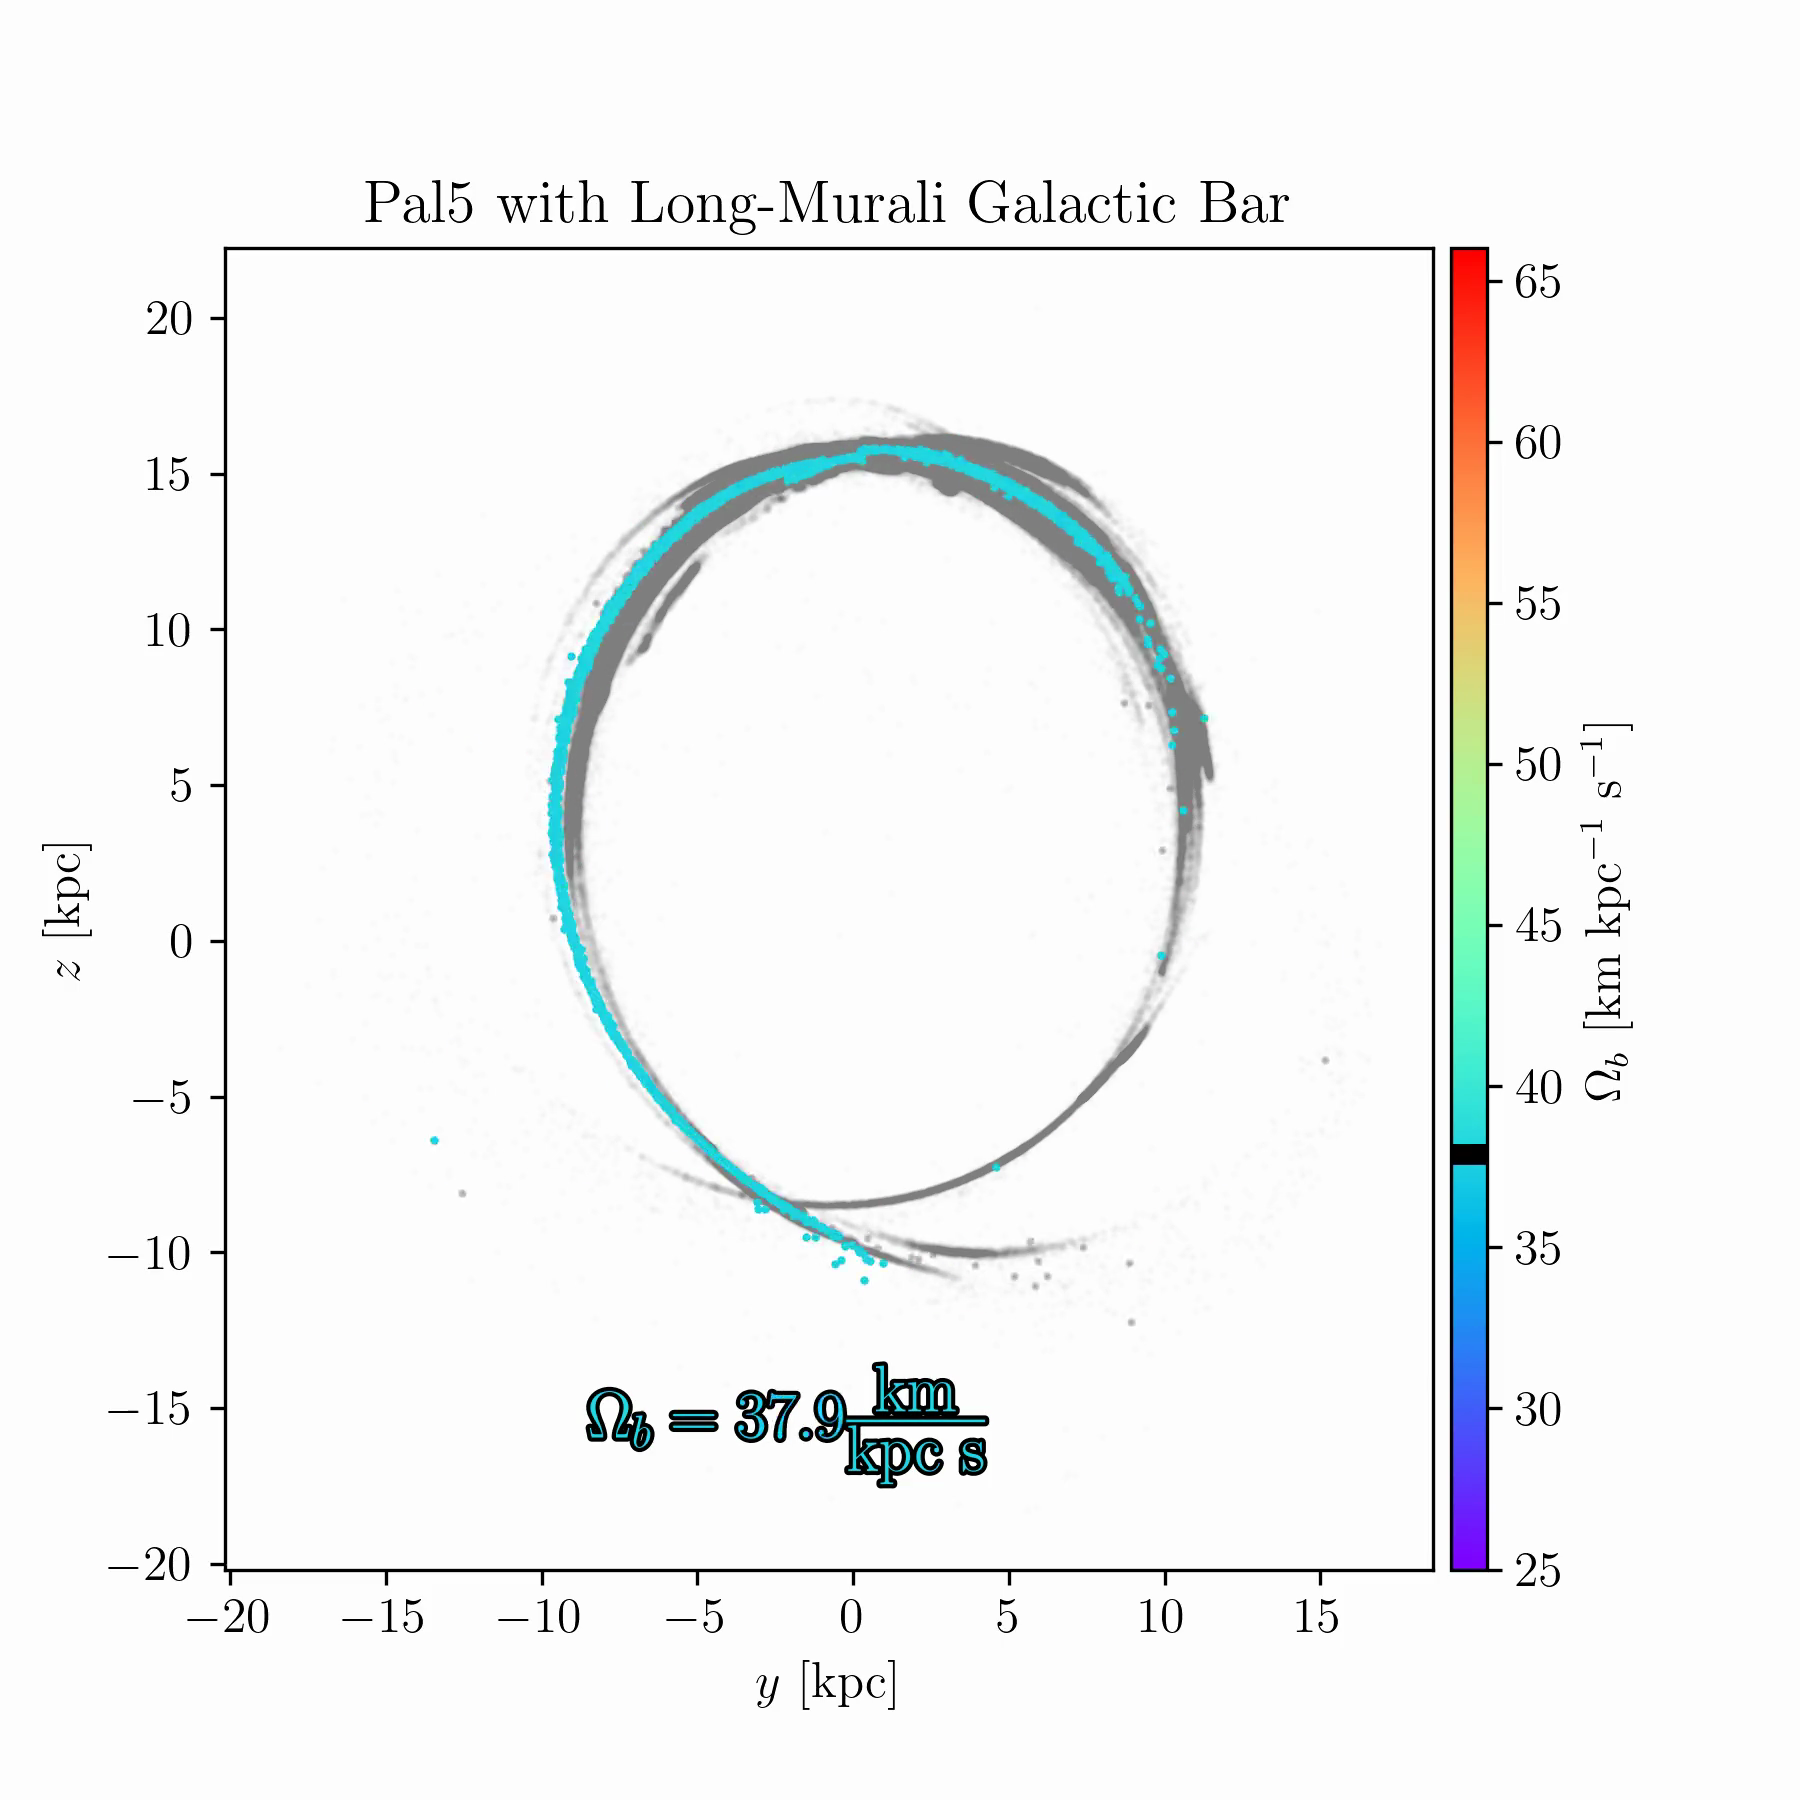
\includegraphics[width=.32\linewidth]{images/frame_0048.png}&
                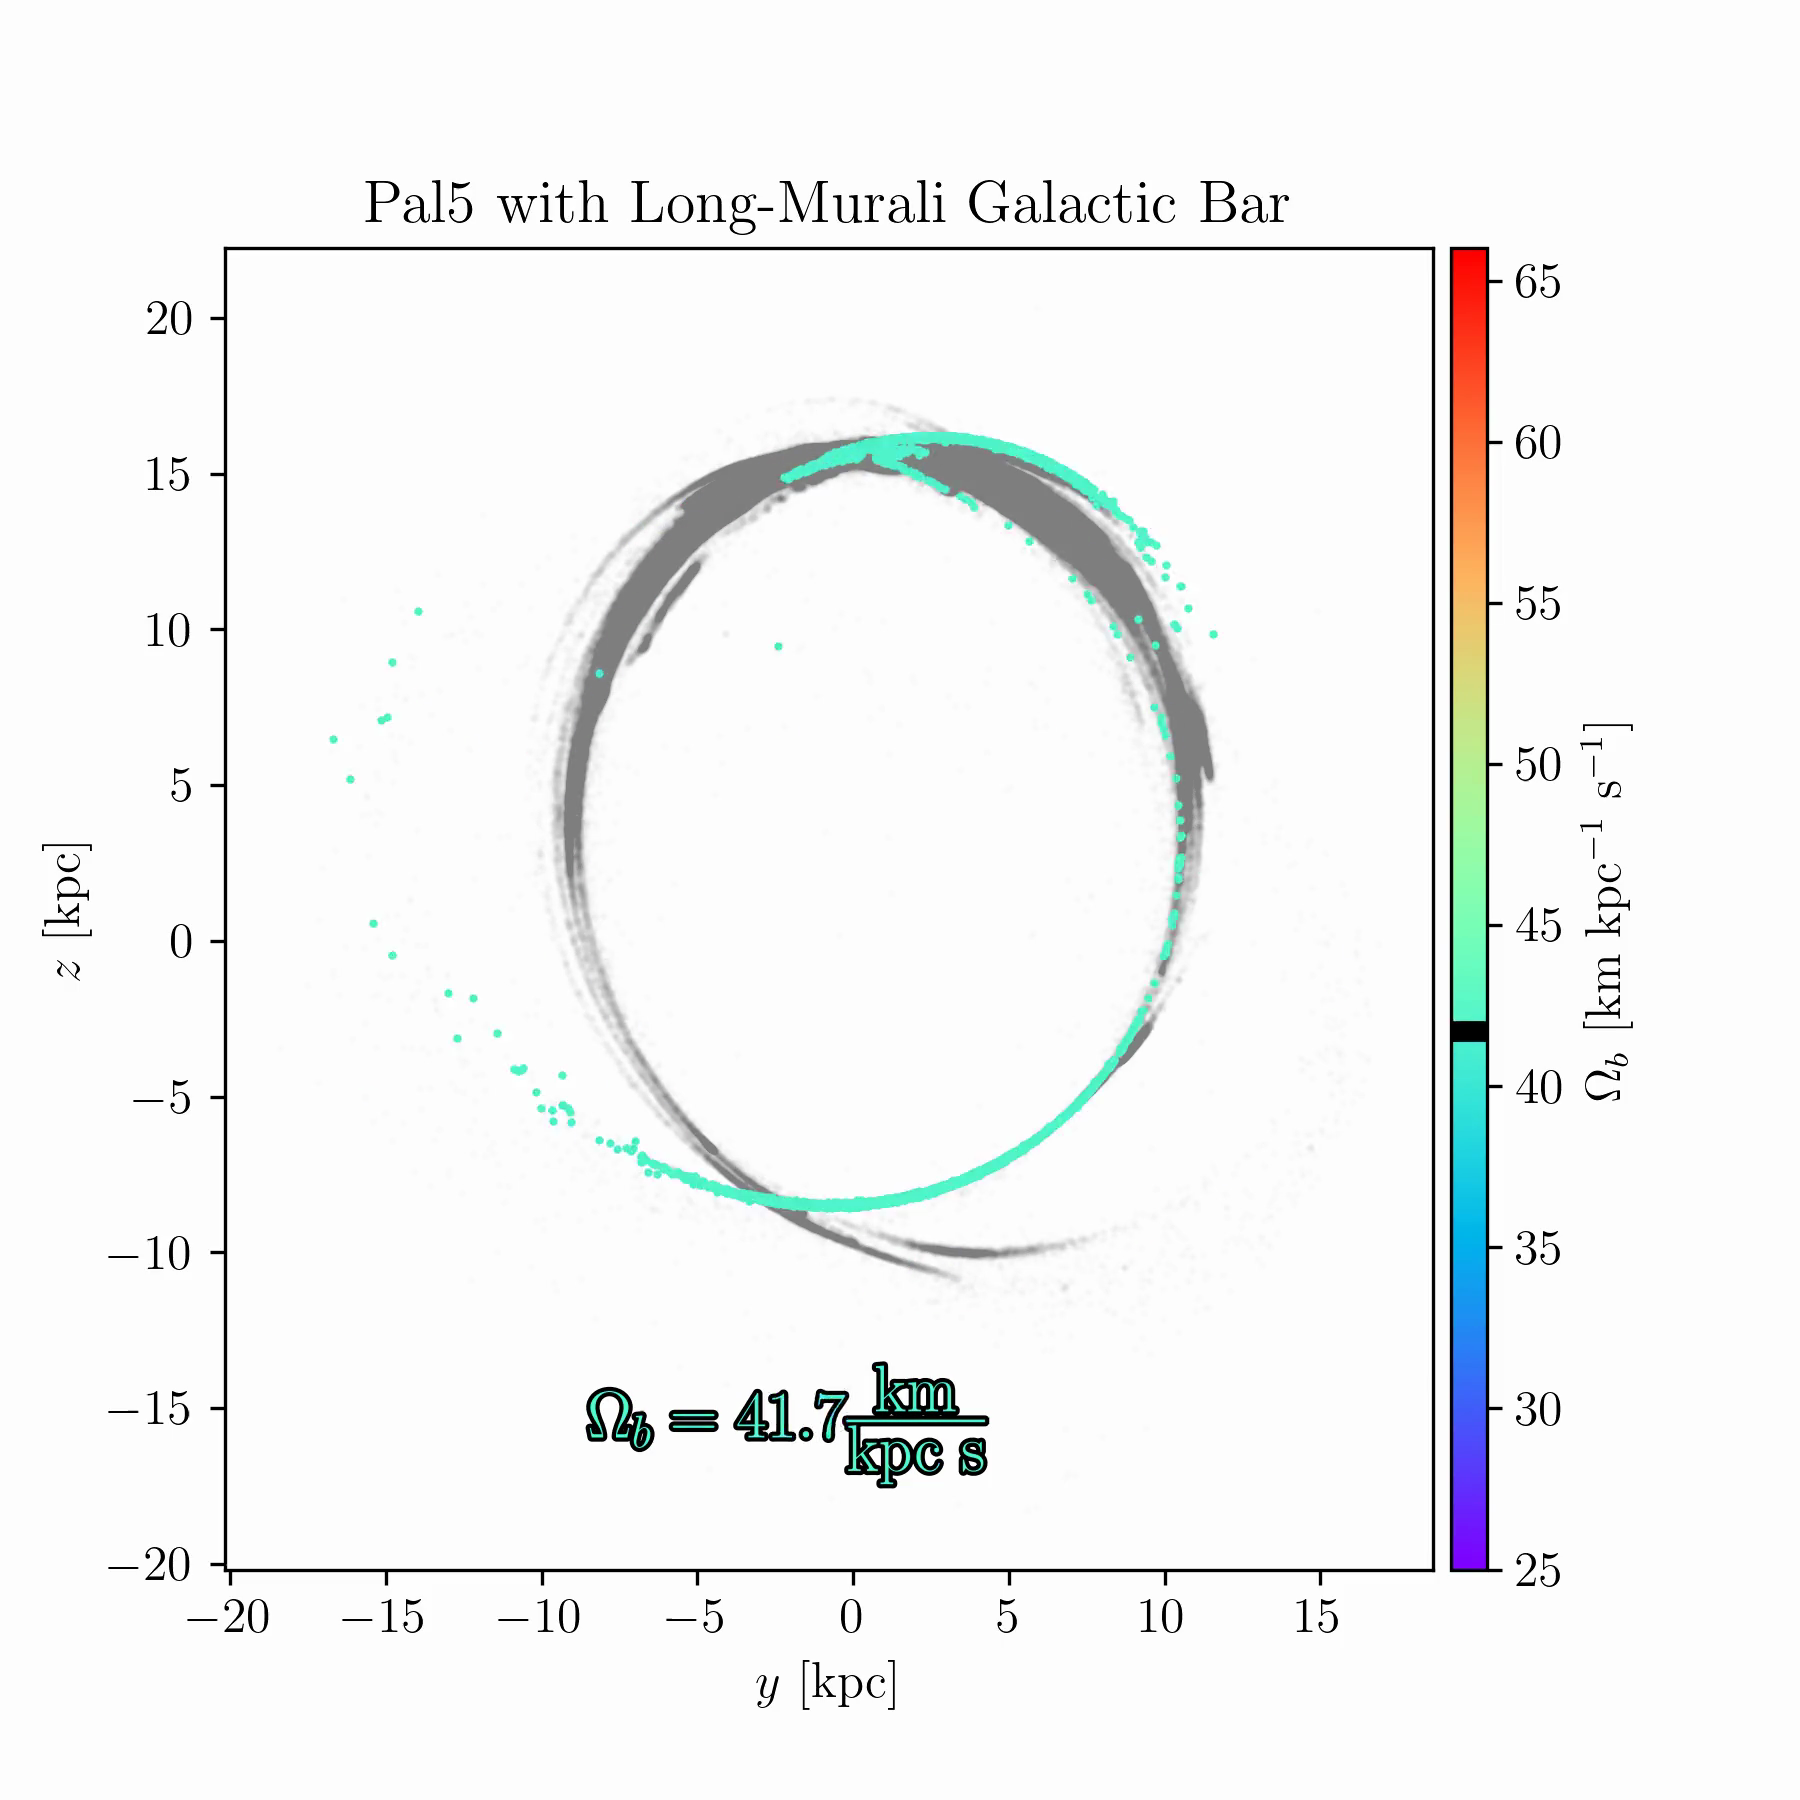
\includegraphics[width=.32\linewidth]{images/frame_0062.png}\\

                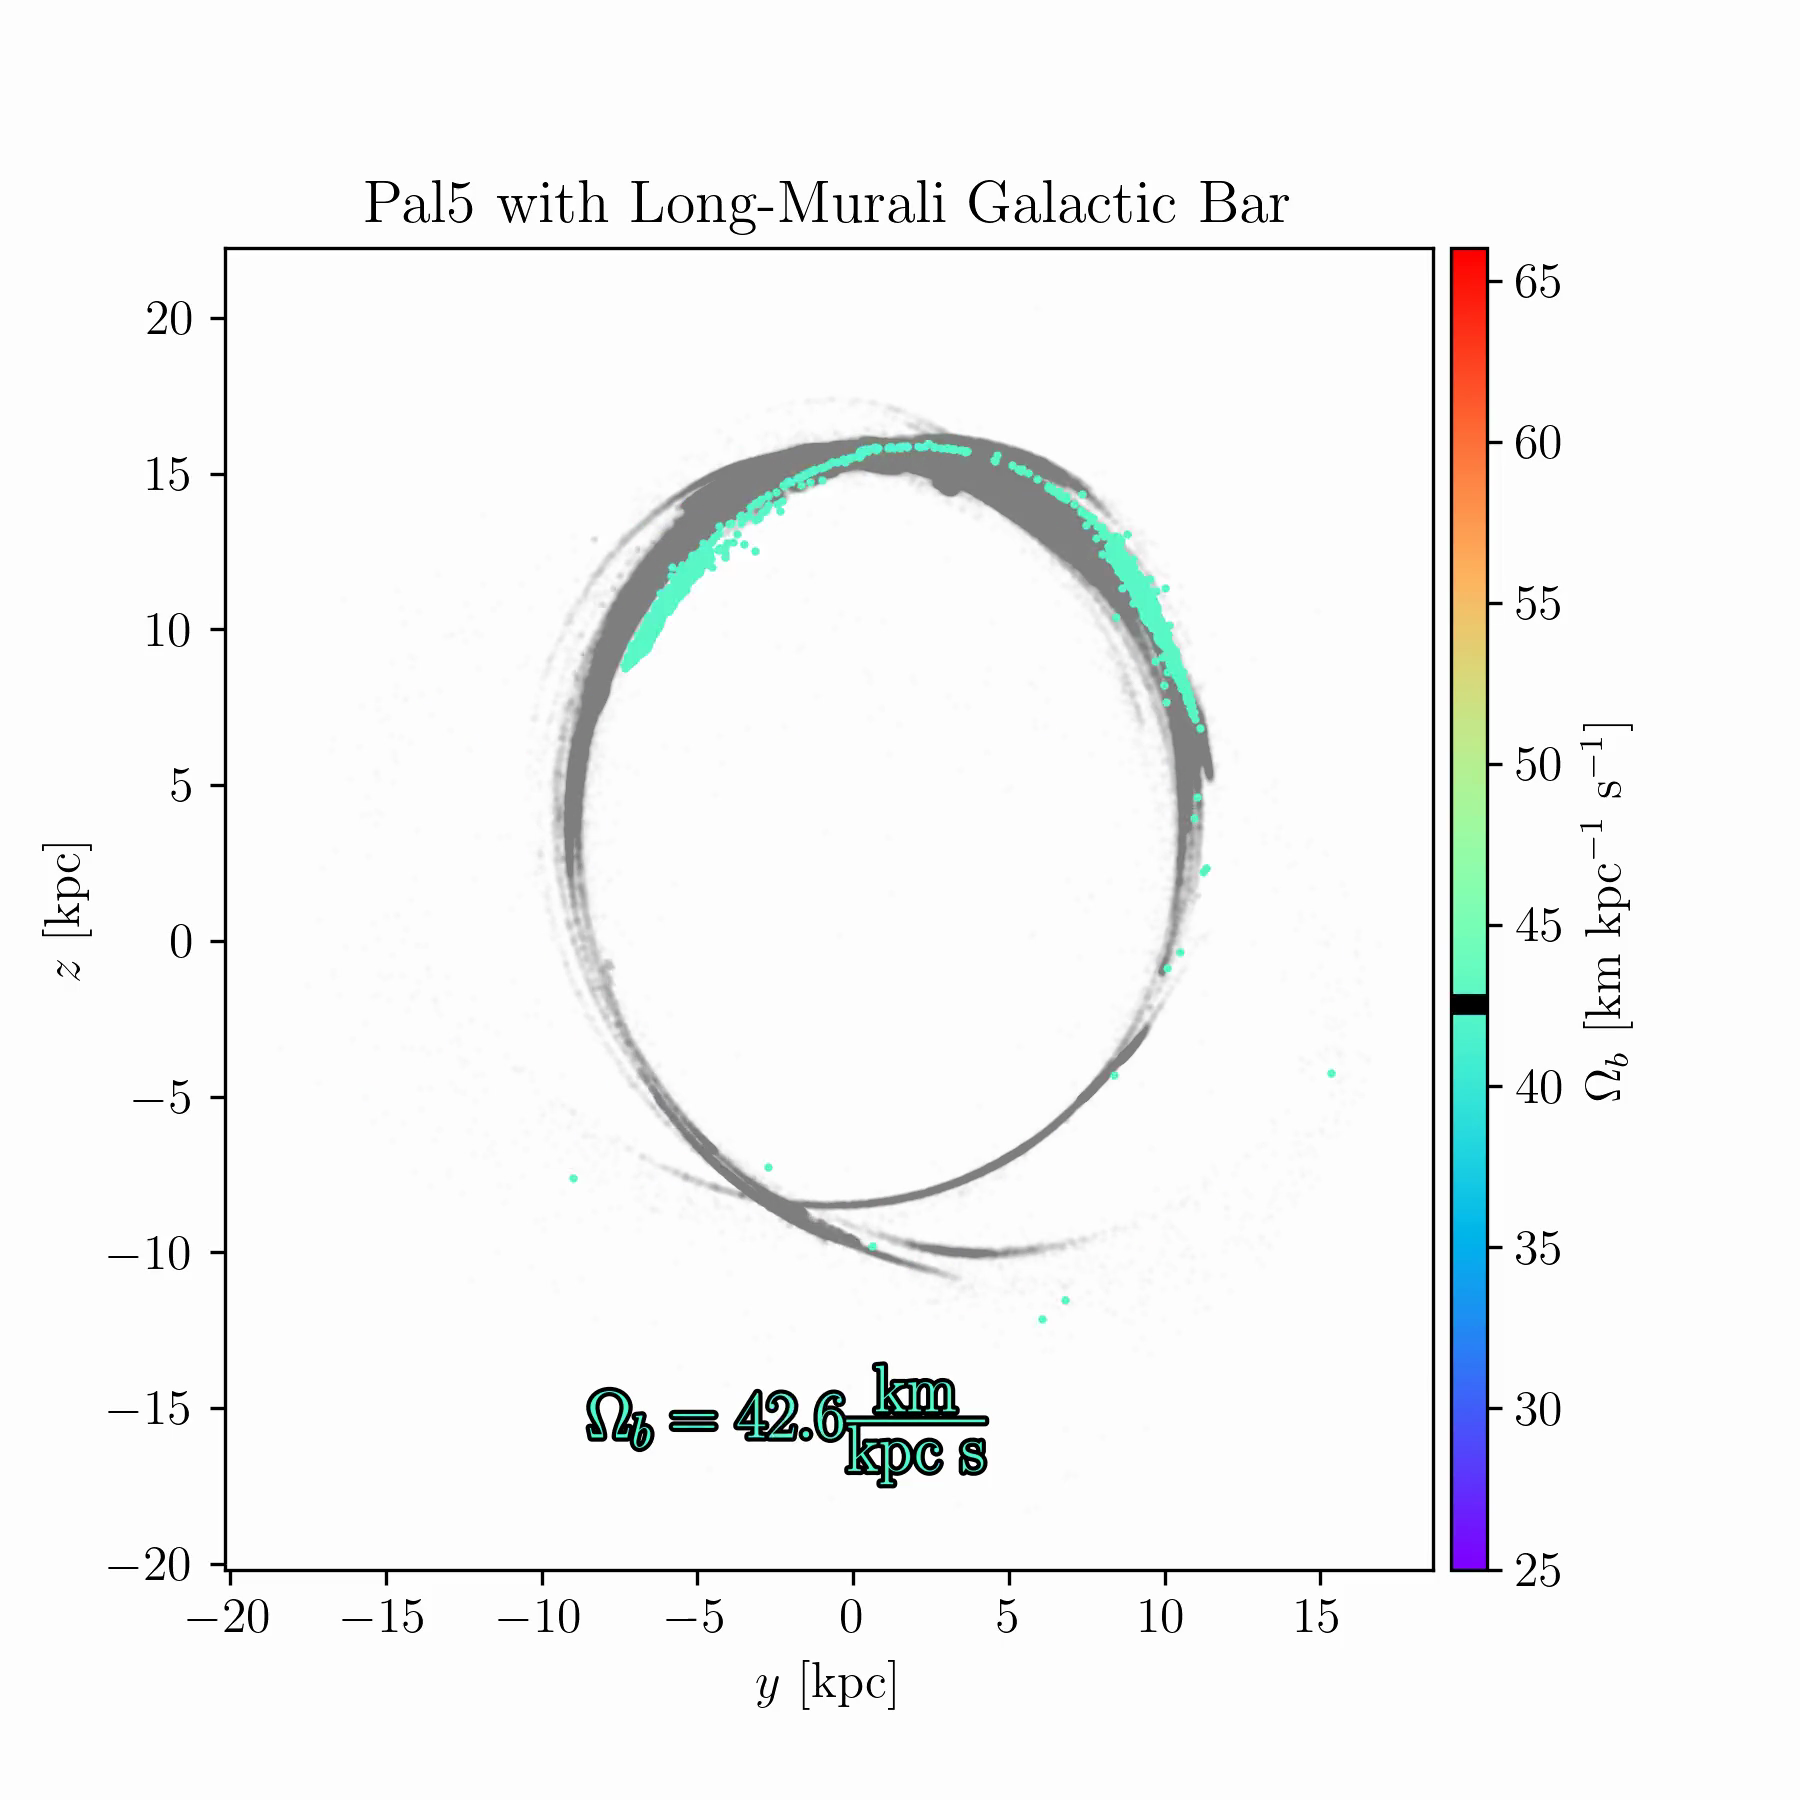
\includegraphics[width=.32\linewidth]{images/frame_0065.png}&
                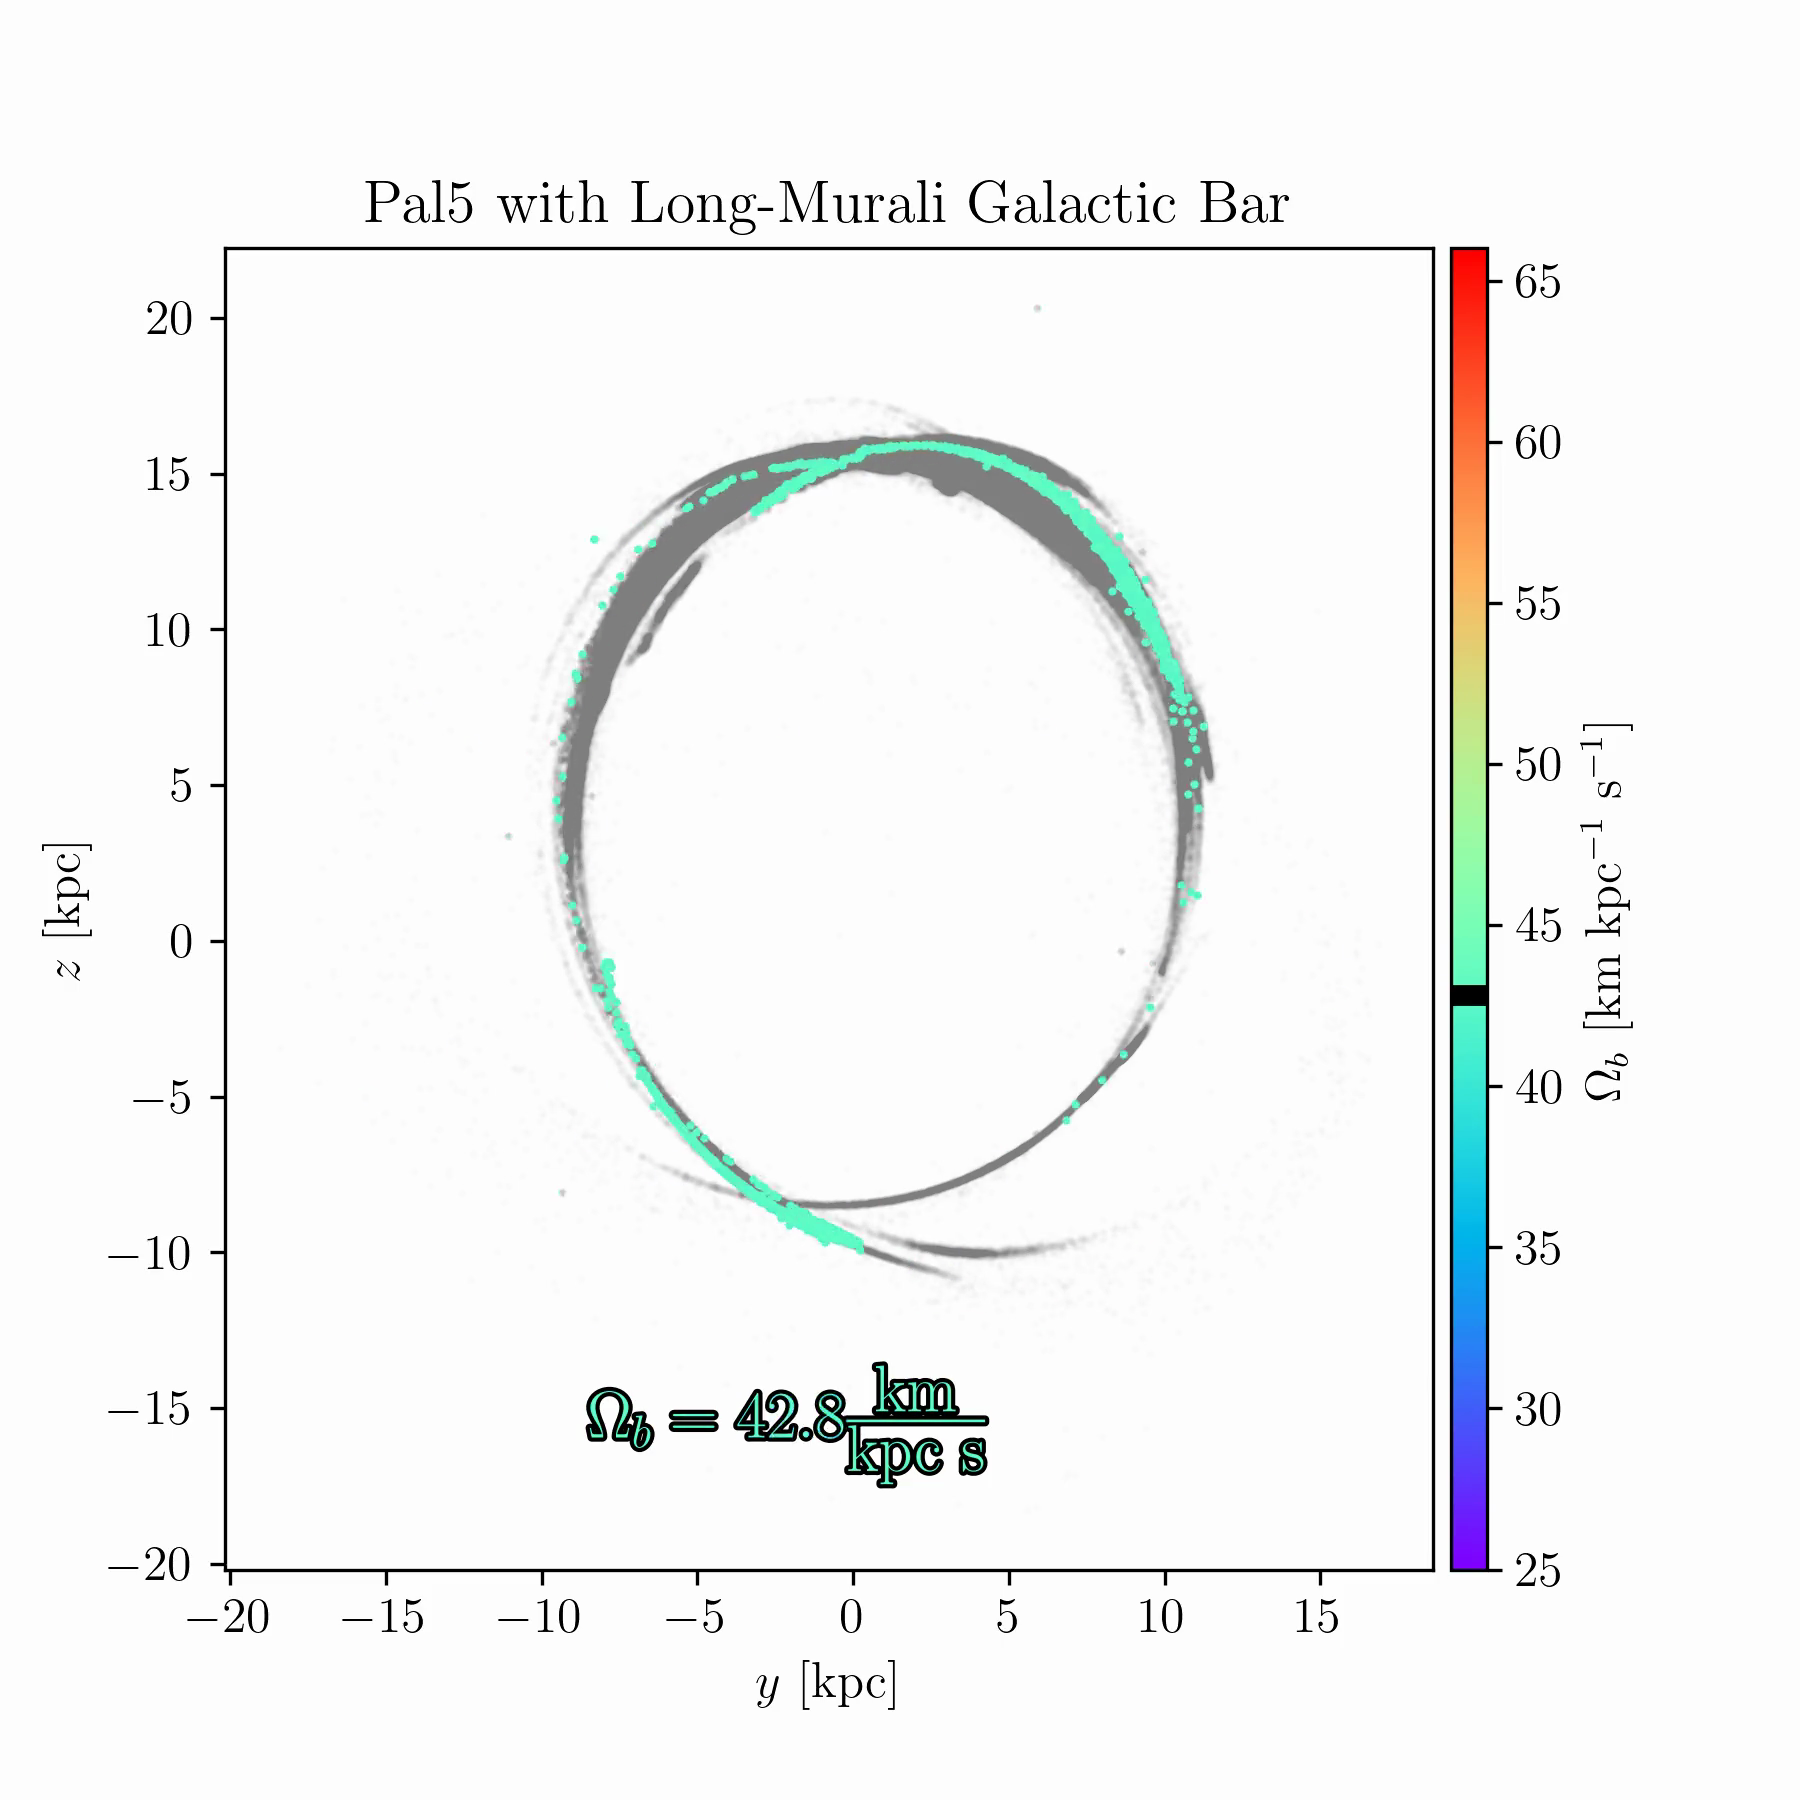
\includegraphics[width=.32\linewidth]{images/frame_0066.png}&
                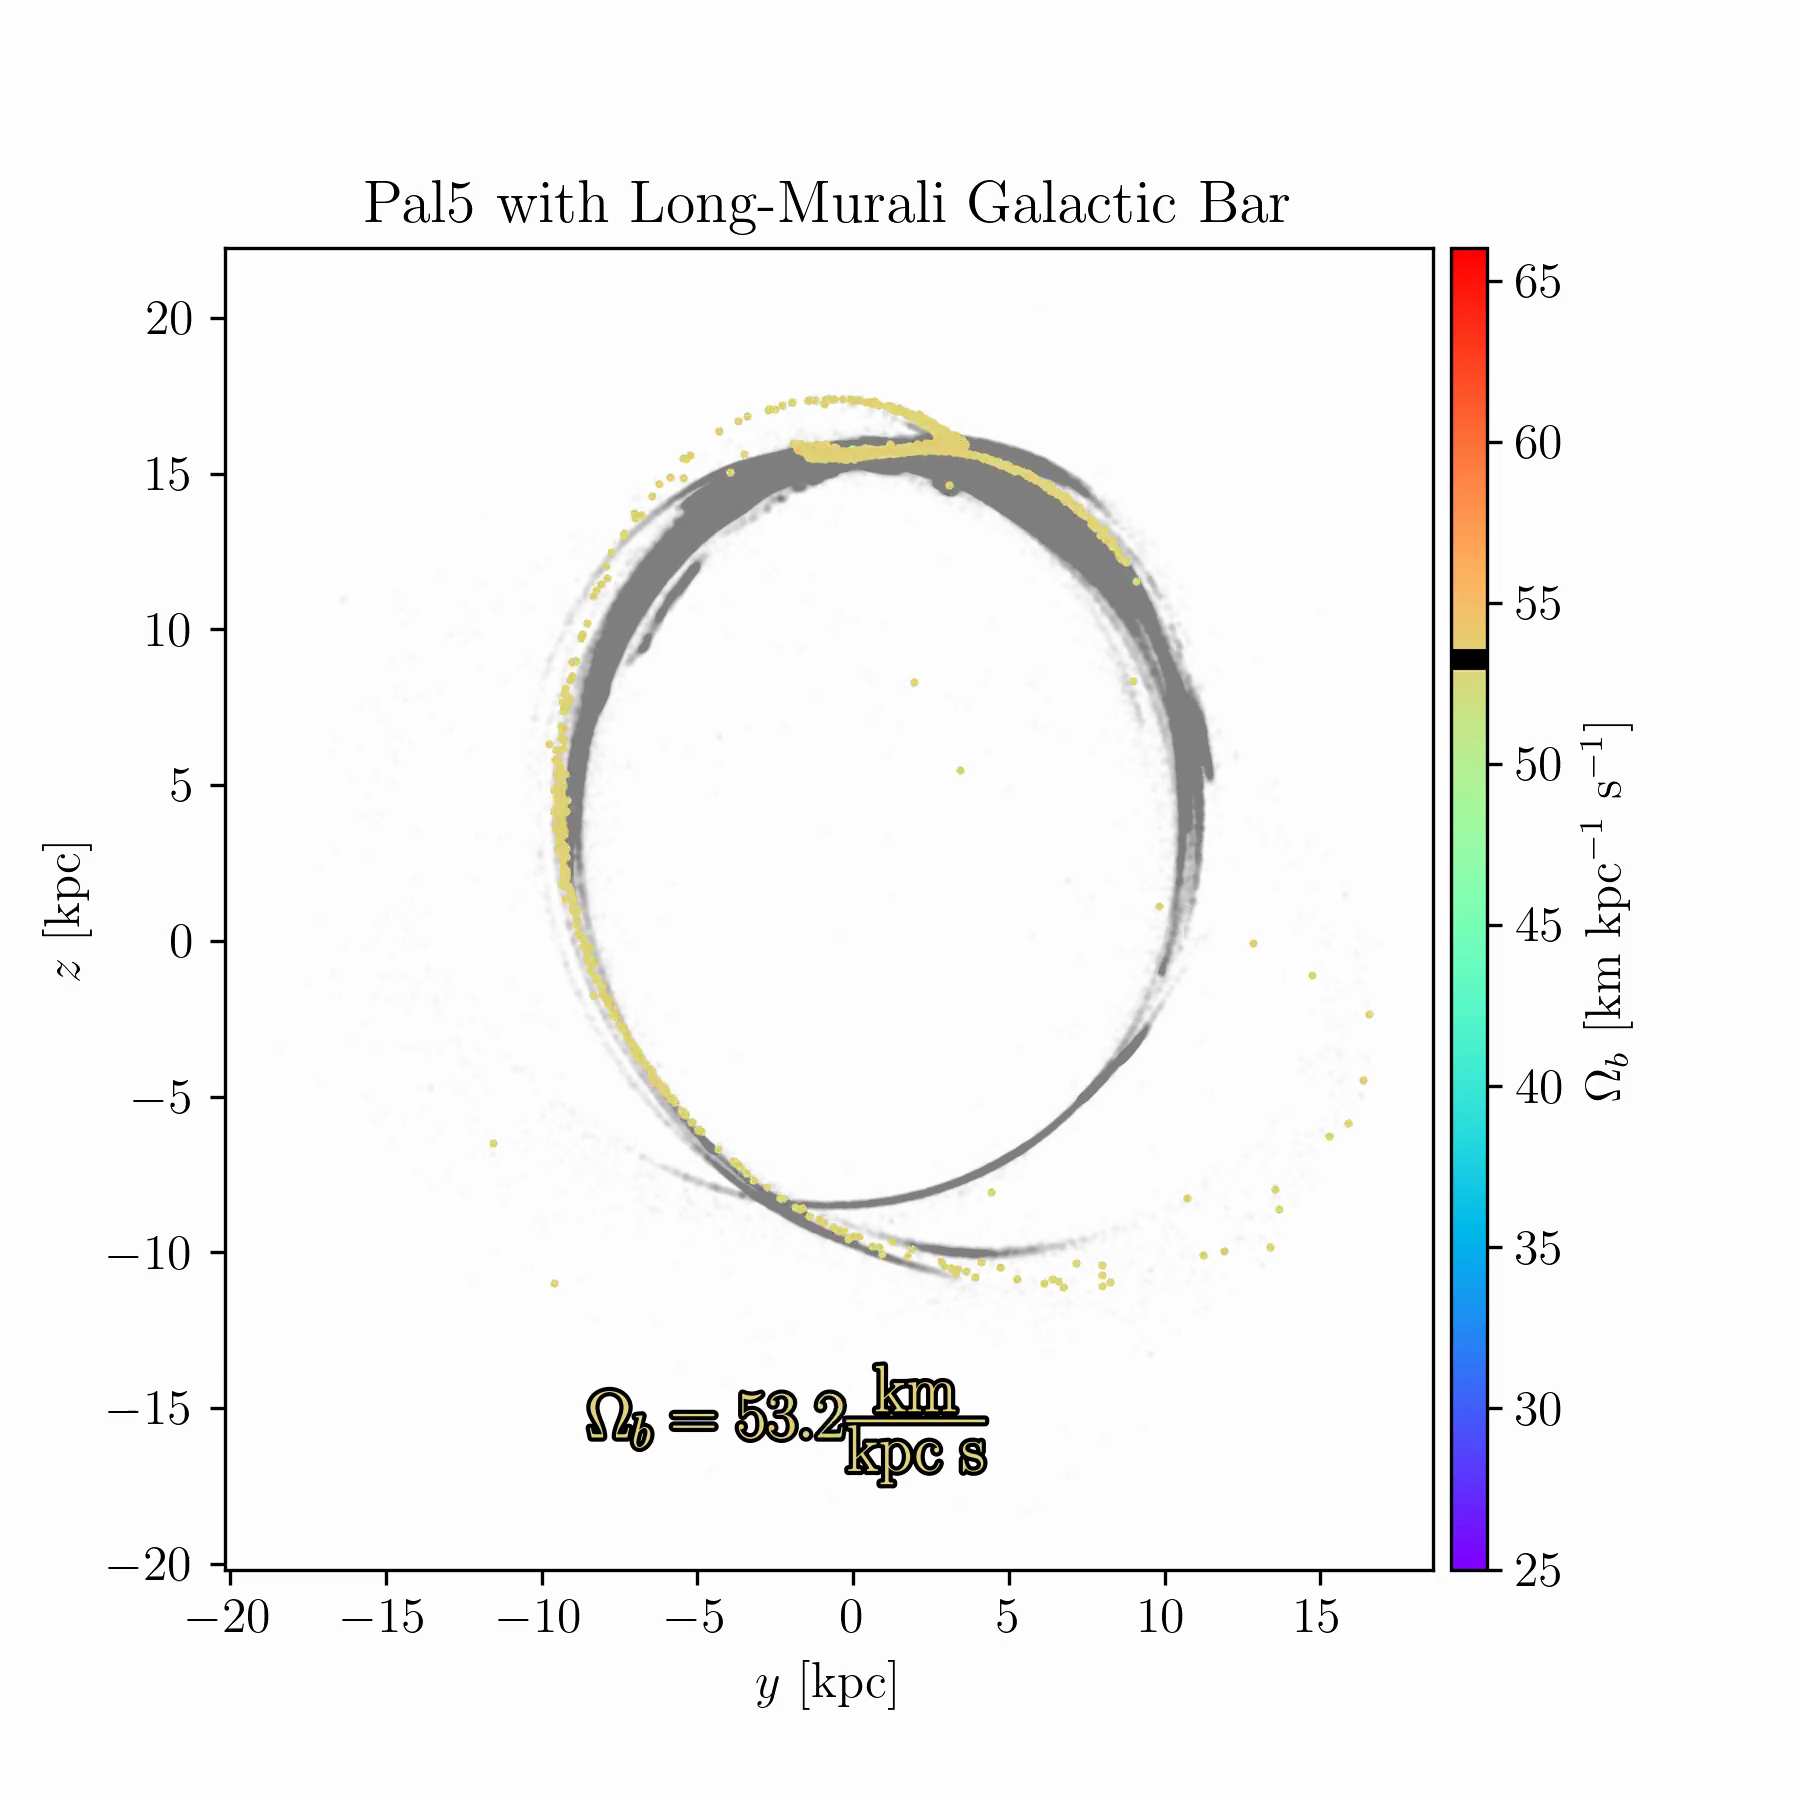
\includegraphics[width=.32\linewidth]{images/frame_0104.png}\\
            \end{tabular}
            \caption[The presence of a stellar bar with different rotational speeds affecting the Palomar~5 stream]{Simulations of the Palomar~5 stream using \texttt{tstrippy} with 5000 particles. The Galactic potential follows \citet{2017A&A...598A..66P} with a bar model from \citet{1997MNRAS.291..717M}, as described in Chapter~4. Palomar~5's initial conditions are identical in all runs, but the bar pattern speed is varied between 25 and 61~km\,s$^{-1}$\,kpc$^{-1}$ over 150 samples. The animated version of this figure is available in the online thesis (Many thanks to Raif Moibi who helped launch and analyze these simulations)}
            \label{fig:pal5_with_bar}
        \end{figure}

        The results in Fig.~\ref{fig:pal5_with_bar} raise several questions. There is room to understand the underlying mechanisms theoretically, and to identify whether any Milky Way globular clusters or streams occupy one of these ``special'' resonances. Such signatures could occur only for a restricted range of bar pattern speeds (or other bar parameters), making them valuable dynamical probes. This is especially important because most existing models of the Milky Way potential, such as that of \citet{2024ApJ...967...89I}, are static and axisymmetric, omitting the bar due to its complexity. If these resonances can be robustly identified in observed streams, they may offer a new route to constraining the Galactic bar and its evolution with time.

    \subsection{Multiple stellar populations, stellar evolution, and globular cluster formation and internal dynamics}
        Globular clusters are peculiar objects. In addition to being massive star clusters, they exhibit distinctive chemical abundance patterns compared to typical Galactic field stars \citep{2012A&ARv..20...50G,2018ARA&A..56...83B,2019A&ARv..27....8G}. Many globular clusters host multiple stellar populations, often interpreted as different generations of star formation. However, no single formation and evolution scenario fully reproduces the observed abundance patterns.

        Some studies have explored dynamical pathways for producing a second generation. For example, \citet{2024A&A...681A..45L} investigated a scenario in which a gaseous disk within a globular cluster forms a second generation of stars. As the disk relaxes into a spherical configuration, the cluster loses roughly 95\% of its mass, resulting in roughly equal numbers of first- and second-generation stars. In this model, material lost to tidal streams is predominantly first-generation.

        While theoretical models link stellar evolution to cluster dynamics, observational studies are beginning to provide kinematic evidence for multiple populations. For instance, \citet{2025MNRAS.537.2342C} measured kinematic differences between two stellar generations in 47 Tuc.        


        Stars with the peculiar chemistry of globular clusters start to be found in all Galactic components, from the halo and bulge \citep{2016ApJ...825..146M,2017MNRAS.465..501S} to the disk, where - for example - \citet{2017ApJ...846L...2F} stars with the characteristic signatures of second-generation cluster members, and \citet{2021ApJ...918L..37F} identified relatively metal-rich cluster debris (still below solar metallicity). This is further evidence that globular cluster mass loss contributed to the Galactic field populations, in an amount which is still difficult to estimate \citep[see, for example][]{2016ApJ...825..146M}.

        Many halo stars share similar chemical patterns with clusters, suggesting that globular clusters may have contributed to the stellar halo \citep{2016ApJ...825..146M,2017MNRAS.465..501S}. There are, however, notable exceptions: \citet{2017ApJ...846L...2F} reported 11 stars with the characteristic signatures of second-generation cluster members within the Galactic disk, and \citet{2021ApJ...918L..37F} identified relatively metal-rich cluster debris in the disk (still below solar metallicity). 

        With improving data quality, it is becoming possible to trace multiple stellar populations beyond the clusters themselves, into their tidal debris \citep{2022MNRAS.510.3727P}. For example, \citet{2024MNRAS.529.2413U} found evidence for multiple populations within a stellar stream not linked to any known cluster. Detailed chemical abundances allowed them to identify the stream as globular cluster debris, even uncovering a star with the distinct chemical fingerprint of a second-generation population.

        In the coming years, as chemical abundance measurements become available for more stars in tidal tails, it may be possible to map the spatial distribution of first- and second-generation stars within streams. Their relative kinematics could provide a direct probe of the progenitor cluster's internal dynamical evolution.

        The models I have presented in this thesis can be enriched by these observations to provide initial constraints on the mass loss history of these clusters.